% !TEX program = xelatex
\let\nofiles\relax
\documentclass{article}
\usepackage{graphicx}
\usepackage{setspace}
% \usepackage{ctex}
\usepackage{indentfirst}
\setlength{\parindent}{2em}  % 用于首行缩进

\usepackage{amsmath}
\usepackage{mathtools}
\usepackage{caption}
\usepackage{subfigure}
\usepackage{amssymb}
\usepackage{amsthm} % 使用定理环境
% \usepackage{ntheorem}
\usepackage{bm}
\usepackage{pdfpages}
\usepackage{multirow}
\usepackage{url}
\usepackage{cite}   % 文献
\usepackage[colorlinks,linkcolor=red,anchorcolor=blue,citecolor=green,CJKbookmarks=True]{hyperref}  % 使用链接 但不用默认属性
% CJKbookmarks让链接支持中文
% \usepackage{hyperref}
% \usepackage{geometry}
% \geometry{a4paper,scale=0.8}
\usepackage{algorithm}
% \usepackage{algorithmic}
\usepackage{geometry}
\geometry{a4paper,left=1in,right=1in,top =1in, bottom = 1in}
\setstretch{1.5}   %  改变行间距
% \newgeometry{left = 2 cm, top= 3 cm}

\title{Dynamic Seat Assignment With Social Distancing}
% \author{Zikang, Li; Xiangtong Qi; Qian Liu}
% \date{}
% \newtheorem{algorithm}{Algorithm}
\newtheorem{thm}{\hspace{2em}Theorem}
\newtheorem{lem}{\hspace{2em}Lemma}
\newtheorem*{pf}{}
% \newtheorem{pf}{Proof}
\newtheorem{remark}{\hspace{2em}Remark}
\newtheorem{corollary}{\hspace{2em}Corollary}
\newtheorem{prop}{\hspace{2em}Proposition}
\newtheorem{definition}{Definition}
\newtheorem{example}{Example}
\DeclareMathOperator{\sign}{sign}
% \newcommand{\sign}{\text{sign}}
\newcommand{\X}{\mathbf{X}}


\begin{document}
\maketitle{}

% !TEX root = sum1.tex

\section*{Abstract}



Keywords: Social Distancing, Seat Assignment, Dynamic Arrival.


% !TEX root = sum1.tex
\section{Introduction}
Social distancing has been a proven concept to contain the spread of an infectious disease. As a general principle, social distancing can be implemented in various forms. The basic requirement of social distancing is the specification of a minimum physical distance between people in public areas. For example, the World Health Organization suggests social distancing by ``keep physical distance of at least 1 meter from others'' (https://www.who.int/emergencies/diseases/novel-coronavirus-2019/advice-for-public). In the US, the CDC refers to social distancing as ``keeping a safe space between yourself and other people who are not from your household.'' (https://stacks.cdc.gov/view/cdc/90522)

Note that under such a requirement, social distancing is actually applied with respect to groups of people. In Hong Kong, the government has adopted social distancing measures, in the recent Covid 19 pandemic, by limiting the size of groups in public gathering to two, four, and six people per group over time. Moreover, the Hong Kong government has also adopted the limit of the total number of people in a venue; for example, restaurants can operate at 50\% or 75\% of their normal seating capacity.


While the above practice of social distancing has been recognized for its primary function,  it is not clear how the entire economy will be affected. This is an important issue in the service sector where social distancing implies fewer clients and lower revenue. The situation is especially complicated under multiple social distancing measures, such as physical distance between groups, limit on the size of groups, and the occupancy rate of the venue. This naturally raises questions regarding the relationship of these measures, e.g., which is relatively more effective under different conditions, whether they compliment or contradict with each other, and more importantly, is it possible to align these measures so that they can be implemented coherently? 

We will address the above issues of social distancing in the context of seating arrangement in a venue, such as a cinema or a conference hall. The venue is equipped with seats of multiple rows.  People come in groups where each group of people will sit consecutively in one row. The social distancing requirement.


% Governments worldwide have been faced with the challenge of reducing the spread of Covid-19 while minimizing the economic impact. Social distancing has been widely implemented as the most effective non-pharmaceutical treatment to reduce the health effects of the virus. 
% This website records a timeline of Covid-19 and the relevant epidemic prevention measures\cite{Covid19Timeline}. For instance, in March 2020, the Hong Kong government implemented restrictive measures such as banning indoor and outdoor gatherings of more than four people, requiring restaurants to operate at half capacity. As the epidemic worsened, the government tightened measures by limiting public gatherings to two people per group in July 2020. As the epidemic subsided, the Hong Kong government gradually relaxed social distancing restrictions, allowing public group gatherings of up to four people in September 2020. In October 2020, pubs were allowed to serve up to four people per table, and restaurants could serve up to six people per table. Specifically, the Hong Kong government also implemented different measures in different venues \cite{Gov202209}. For example, the catering businesses will have different social distancing requirements depending on their mode of operation for dine-in services. They can operate at 50\%, 75\%, or 100\% of their normal seating capacity at any one time, with a maximum of 2, 2, or 4 people per table, respectively. Bars and pubs may open with a maximum of 6 persons per table and a total number of patrons capped at 75\% of their capacity. The restrictions on the number of persons allowed in premises such as cinemas, performance venues, museums, event premises, and religious premises will remain at 85\% of their capacity.


The measures implemented by the Hong Kong government primarily concentrate on restricting social distancing, group sizes and occupancy rates. However, implementing these policies in practice can pose challenges, particularly for fixed seating layouts with dynamic arrivals of people. In the original commercial case without social distancing requirements, customers did not need to sit together, so the focus was solely on total capacity. Under social distancing constraints, placing groups in row runs the risk of being unable to find matching demand, potentially leaving empty seats.

To avoid confusion, we clarify the distinction between `seat planning' and `seat assignment' which will be used in the following parts. In our context, the seat planning means the seat partition in the planning. The planning can be altered later when the planned seats don't match with the size of a coming group or when the seat planning is disrupted after assigning a coming group. In the seat assignment, for the coming group, when accepting it, we assign the seats to the group, and the seats will not be used by others in the future.

In order to adhere to social distancing guidelines, it is important to understand the process of generating seat planning based on known groups and how to assign seats to incoming groups. Additionally, it is of interest to explore how the social distancing constraints impact the sellers and the specific policies formulated by the government to address social distancing concerns.

We intend to shed light on the problem just described and to propose the practical dynamic seat assignment policy. In particular, we investigate the following questions. 

1. How can we model the seat planning problem given the social distancing restrictions? What kind of property does this problem have? How can we give a seat planning to accommodate the maximum people with stochastic demand?

2. How to use the property of seat planning problem to design the dynamic seat assignment policy? How good is the performance of this policy compared with other policies?

3. What kind of insights regarding the social distancing and occupancy rates can we obtain when implementing the dynamic seat assignment policy?

% In our study, we will focus on addressing this challenge in commercial premises, such as cinemas and music concert venues. We aim to provide a practical tool for venues to optimize seat assignments by proposing a seat assignment policy that takes into account social distancing requirements and the given seat layout. We strive to enable venues to implement social distancing measures effectively by offering a solution that provides specific seating arrangements.

To answer these questions, we construct the seat planning problem with deterministic and stochastic demand under social distancing requirement. For the deterministic situation, we have complete and accurate information about the demand for seating. We aim to provide a seat planning that maximizes the number of people accommodated. This situation is applicable in venues like churches or company meetings, where fixed seat layouts are available, and the goal is to assign seats to accommodate as many people as possible within the given layout. The seat planning obtained shows the utilization of as many seats as possible. Thus, we introduce the concept of full or largest pattern to indicate the seat partition of each row. For the seat planning that does not utilize all available seats, we propose to improve the seat planning by incorporating full or largest patterns.

For the stochastic situation, we have knowledge of the demand distribution before the actual demand is realized. We aim to generate a seat planning that maximizes the expected number of people accommodated. This approach is suitable for venues where seats have been pre-allocated to ensure compliance with social distancing rules. With the given demand scenarios, we develop the scenario-based stochastic programming to obtain the seat planning. To solve this problem efficiently, we apply the Benders decomposition technique. However, in some cases, solving the integer programming with Benders decomposition remains still computationally prohibitive. Thus, we can consider the LP relaxation then obtain a feasible seat planning by deterministic model. Based on that, we construct a seat planning composed of full or largest patterns to fully utilize all seats.

We mainly focus on addressing the dynamic seat assignment problem with a given set of seats in the context of social distancing. Solving the problem by dynamic programming can be prohibitive due to the curse of dimensionality, which arises when the problem involves a large number of variables or states. To mitigate this complexity, we begin by generating a seat planning in the stochastic situation. This seat planning acts as a foundation for the seat assignment. Then, we develop the dynamic seat assignment policy which guides the allocation of seats to the incoming groups sequentially. In the numerical result, our policy performs well compared with other policies. 
We use $\tilde{T}$ to denote the gap point, which refers to the first time period at which, on average, the number of people accepted without social distancing is not less than that accepted with social distancing plus one. By sampling many probability combinations, the results show that $\tilde{T}$ and the corresponding occupancy rate, $\beta(\tilde{T})$, can be estimated with $\gamma$, the expected number of people per period. Different $\gamma$ corresponds to different $\tilde{T}$. When the total number of periods, $T$, is less than $\tilde{T}$, we tend to accept all incoming groups. In this case, there is no difference whether to implement the social distancing restriction. When $T$ is larger, there will be more groups rejected when implementing the social distancing requirement. The government can consider the potential losses when making policies regarding group size and occupancy rate. Similarly, the seller can implement corresponding measures to adhere to these requirements.

% Regarding the seat assignment with social distancing constraint, we consider the dynamic demand based on the seat planning. For the dynamic situation, the decision to accept or reject a group is made for each incoming group. This situation is commonly encountered in venues such as cinemas or music concerts, where decisions can be made on a group-by-group basis. The goal is to make timely decisions regarding seat assignments, considering factors such as available seating capacity, social distancing requirements and the specific size of each group.

% The following figures illustrate the seat planning and seat assignment. 

% \begin{figure}[htbp]
%     \centering
%     \begin{minipage}[t]{0.48\textwidth}
%     \centering
%     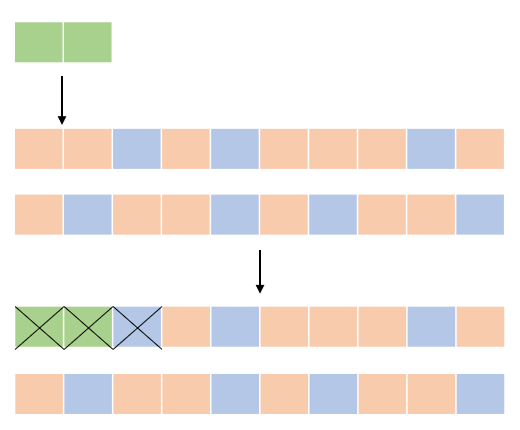
\includegraphics[width=5cm]{./Figures/seat_assign1.png}
%     \caption{Assign The Group in Row 1}
%     \end{minipage}
%     \begin{minipage}[t]{0.48\textwidth}
%     \centering
%     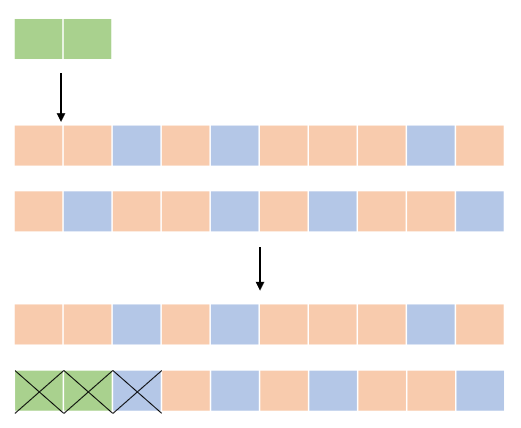
\includegraphics[width=5cm]{./Figures/seat_assign2.png}
%     \caption{Assign The Group in Row 2}
%     \end{minipage}
% \end{figure}


Our main contributions in this paper are summarized as follows. First, this study presents the first attempt to consider the arrangement of seat assignments with social distancing under dynamic arrivals. While many studies in the literature highlight the importance of social distancing in controlling the spread of the virus, they often focus too much on the model and do not provide much insight into the operational significance behind social distancing \cite{barry2021optimal, fischetti2021safe}. Recent studies have explored the effects of social distancing on health and economics, mainly in the context of aircraft \cite{salari2020social, ghorbani2020model, salari2022social}. Our study provides a new perspective to help the government adopt a mechanism for setting seat assignments to implement social distancing during pandemic.

Second, we establish a deterministic model to analyze the effects of social distancing when the demand is known. Due to the medium size of the problem, we can solve the IP model directly. We then develop the scenario-based stochastic programming by considering the stochastic demands of different group types. By using Benders decomposition methods, we can obtain the seat planning quickly. 

Third, to address the problem in the dynamic situation, we first obtain a feasible seat planning from scenario-based stochastic programming. We then make a decision for each incoming group based on our dynamic seat assignment policy, either accepting or rejecting the group. Our results demonstrate a significant improvement over the traditional control policies and provide the insights on the implementation of social distancing.

% Our results demonstrate the effectiveness of our approach in balancing social distancing requirements with revenue generation, providing valuable insights for policymakers and venue managers. Specifically, our proposed approach can help cinemas, concert venues, and other public spaces optimize seat assignments while ensuring the safety of patrons. It provides a practical tool for venues to implement social distancing measures in a flexible and efficient manner, adapting to changes in demand and maximizing revenue generation while maintaining social distancing measures.

% With this new .., we illustrate how to assign the seats by the govenment/stakeholder to balance health and economic issues. In addition, we also provide managerial guidance for the government on how to publish the related policy to make the tradeoff between economic maintenance and risk management.

The rest of this paper is structured as follows. The following section reviews relevant literature. We describe the motivating problem in Section 3. In Section 4, we establish the stochastic model,analyze its properties and obtain the seat planning. Section 5 demonstrates the dynamic seat assignment policy to assign the seats for incoming groups. Section 6 gives the numerical results and the insights of implementing social distancing. The conclusions are shown in Section 7.
\newpage


% !TEX root = sum1.tex
\section{Literature Review}

The present study is closely connected to the following research areas -- seat planning with social distancing and dynamic seat assignment. The subsequent sections review literature pertaining to each perspective and highlight significant differences between the present study and previous research.


\subsection{Seat Planning with Social Distancing}
Since the outbreak of covid-19, social distancing is a well-recognized and practiced method for containing the spread of infectious diseases \cite{moosa2020effectiveness}. An example of operational guidance is ensuring social distancing in seat plannings.
% particularly in social distancing measures that involve operational details. 

Social distancing in seat planning has attacted considerable attention from the research area. The applications include the allocation of seats on airplanes \cite{ghorbani2020model}, classroom layout planning \cite{bortolete2022support}, seat planning in long-distancing trains \cite{haque2022optimization}. The social distancing can be implemented in various forms, such as fixed distances or seat lengths. Fischetti et al.\cite{fischetti2021safe} consider how to plant positions with social distancing in restaurants and beach umbrellas. Different venues may require different forms of social distancing; for instance, on an airplane, the distancing between seats and the aisle must be considered \cite{salari2022social}, while in a classroom, maximizing social distancing between students is a priority \cite{bortolete2022support}.

These researchs focus on the static version of the problem. This typically involves creating an IP model with social distancing constraints \cite{bortolete2022support, ghorbani2020model, haque2022optimization}, which is then solved either heuristically or directly. The seat allocation of the static form is useful for fixed people, for example, the students in one class. But it is not be practical for the dynamic arrivals in commercial events.


% and family-group seat selection in a theater. \cite{fischetti2021safe}


% Dynamic seat assignment with social distancing can be implemented manually by the venue staff, or through automated systems that use algorithms to optimize the seating arrangements based on various factors, such as the number of available seats, customer preferences, and the recommended distancing between audience members.

% \subsection{Group seat reservation}
The recent pandemic has shed light on the benefits of group reservations, as they have been shown to increase revenue without increasing the risk of infection \cite{moore2021seat}. In our specific setting, we require that groups be accepted on an all-or-none basis, meaning that members of the same family or group must be seated together. However, the group seat reservation policy poses a significant challenge when it comes to determining the seat assignment policy.


This group seat reservation policy has various applications in industries such as hotels \cite{li2013modeling}, working spaces\cite{fischetti2021safe}, public transport\cite{deplano2019offline}, sports arenas\cite{kwag2022optimal}, and large-scale events \cite{lewis2016creating}. This policy has significant impacts on passenger satisfaction and revenue, with the study \cite{yuen2002group} showing that passenger groups increase revenue by filling seats that would otherwise be empty. Traditional works \cite{clausen2010off, deplano2019offline}in transportation focus on maximizing capacity utilization or reducing total capacity needed for passenger rail, typically modeling these problems as knapsack or binpacking problems.

Some related literature mentioned the seat planning under pandemic for groups are represented below.
Fischetti et al. \cite{fischetti2021safe} proposed a seating planning for known groups of customers in amphitheaters. Haque and Hamid \cite{haque2022optimization} considers grouping passengers with the same origin-destination pair of travel and assigning seats in long-distance passenger trains. Salari et al. \cite{salari2022social} performed group seat assignment in airplanes during the pandemic and found that increasing passenger groups can yield greater social distancing than single passengers. Haque and Hamid \cite{haque2023social} aim to optimize seating assignments on trains by minimizing the risk of virus spread while maximizing revenue. The specific number of groups in their models is known in advance. But in our study, we only know the arrival probabilities of different groups.

This paper \cite{blom2022filling} discusses strategies for filling a theater by considering the social distancing and group arrivals, which is similar to ours. However, unlike our project, it only focuses on a specific location layout and it is still based on a static situation by giving the proportion of different groups.

% In contrast, there is a lack of research on group seat reservations for booking tickets for cinemas, where available seats are typically displayed for customers to choose from for low-demand movie tickets. For concerts with high demand, it is usually not possible to choose seats independently, and the organizer will inform seat information after confirming the order. 
% For movies of the same time period, the ticket prices are the same, while for the same concert, although there are different ticket prices, for the same region, the ticket prices are the same. Therefore, we can consider different ticket prices separately. 
% In the absence of an epidemic, all requests for tickets can be considered one by one. However, the COVID-19 pandemic has shed new light on the potential benefits of group reservations, as they can improve revenue without increasing the risk of infection. 


% Dundar and Karakose \cite{dundar2021seat} proposed a two-stage algorithm for classroom seat assignment during the pandemic, with the first phase maximizing total allocations and the second phase maximizing the minimum interpersonal distance between students. 


\subsection{Dynamic Seat Assignment}
Our model in its static form can be viewed as a specific instance of the multiple knapsack problem \cite{pisinger1999exact}, where we aim to assign a subset of groups to some distinct rows. 


In our dynamic form, the decision to accept or reject groups is made at each stage as they arrive. The related problem can be dynamic knapsack problem \cite{kleywegt1998dynamic}, where there is one knapsack.

% and dynamic bin-packing problem \cite{coffman1983dynamic, berndt2020fully} where items arrive and depart online and all knapsacks are the same. 

% However, solving this problem is strongly NP-hard, which means that finding an optimal solution for large instances of the problem is computationally challenging \cite{pisinger1999exact}.

Dynamic seat assignment is a process of assigning seats to passengers on a transportation vehicle, such as an airplane, train, or bus, in a way that maximizes the efficiency and convenience of the seating arrangements \cite{hamdouch2011schedule, berge1993demand, zhu2023assign}. 

Our problem is closely related to the network revenue management (RM) problem \cite{williamson1992airline}, which is typically formulated as a dynamic programming (DP) problem. However, for large-scale problems, the exponential growth of the state space and decision set makes the DP approach computationally intractable. To address this challenge, we propose using scenario-based programming \cite{feng2013scenario, casey2005scenario, henrion2018problem} to determine the seat planning. In this approach, the aggregated supply can be considered as a protection level for each group type. Notably, in our model, the supply of larger groups can also be utilized by smaller groups. This is because our approach focuses on group arrival rather than individual unit, which sets it apart from traditional partitioned and nested approaches \cite{curry1990optimal, van2008simulation}.


We have two distinct features: group-based and assignment.

Traditional revenue management focuses on decision-making issues, namely accepting or rejecting a request \cite{gallego1997multiproduct}.However, our paper not only addresses decision-making, but also emphasizes the significance of assignment, particularly in the context of seat assignment. This sets it apart from traditional revenue management methods and makes the problem more challenging.

Similarly, the assign-to-seat feature introduced by Zhu et al. \cite{zhu2023assign} also highlights the importance of seat assignment in revenue management. This trait addresses the challenge of selling high-speed train tickets in China, where each request must be assigned to a single seat for the entire journey and takes into account seat reuse. This further emphasizes the significance of seat assignment and sets it apart from traditional revenue management methods.


% The authors propose a modified network revenue management model and introduce a bid-price control policy based on a novel maximal sequence principle. They also propose a "re-solving a dynamic primal" policy that achieves uniformly bounded revenue loss. The study reveals connections between this problem and traditional network revenue management problems and shows that the impact of the assign-to-seat restriction can be limited with the proposed methods.


% Jiang et al. \cite{jiang2015dynamic} proposes a revenue management approach for high-speed rail (HSR) passenger ticket assignment with dynamic adjustments. The approach integrates short-term demand forecasting, ticket assignment, and dynamic ticket adjustment mechanisms to allocate passenger tickets during presale periods and avoid situations where tickets are insufficient at some stations while seats remain empty.



% Implementing dynamic seat assignment with social distancing can be done manually by the staff or through automated systems that use algorithms to optimize the seat assignments based on various factors, such as ticket sales, seat availability, and customer preferences. However, the implementation of social distancing measures poses unique challenges that require careful planning and consideration of various factors to balance safety with revenue generation.


% \subsection{Scenario generation}

% It is challenging to consider all the possible realizations; thus, it is practicable to use discrete distributions with a finite number of scenarios to approximate the random demands. This procedure is often called scenario generation.

% Some papers consider obtaining a set of scenarios that realistically represents the distributions of the random parameters but is not too large. \cite{feng2013scenario} \cite{casey2005scenario}
% \cite{henrion2018problem}

% Another process to reduce the calculation is called scenario reduction. It tries to approximate the original scenario set with a smaller subset that retains essential features.



% Every time we can regenerate the scenario based on the realized demands. (Use the conditional distribution or the truncated distribution)


% Suppose that the groups arrive from small to large according to their size. Once a larger group comes, the smaller one will never appear again.

% When a new group arrives (suppose we have accepted $n$ groups with the same size), we accept or reject it according to the supply (when $n+1 < \text{supply}$, we accept it). 
% then update the scenario set according to the truncated distribution. We can obtain a new supply with the new probability and scenario set.


\newpage


% !TEX root = sum1.tex
\section{Problem Description}
In this section, to incorporate the social distancing into seat planning, we first give the description of the seat planning problem with social distancing. Then we introduce the dynamic seat assignment problem with social distancing.

% dynamic seat assignment problem, which is suitable for commercial use in cinemas and concerts.

\subsection{Seat Planning Problem with Social Distancing}\label{dynamic_demand}
We consider a set of groups, each of which consists of no more than $M$ people, to be assigned to a set of seats. There are $M$ different group types, with group type $i$ containing $i$ people, where $i \in \mathcal{M} \coloneqq \{1,2, \ldots, M\}$. (We use $\mathcal{M} = \{1, \ldots, M\}$ to denote the set of all positive integers that are no larger than $M$.)

These groups can be represented by a demand vector, denoted by $\mathbf{d} = [d_1, \ldots, d_M]$. Each element $d_i$, where $i \in \mathcal{M}$, indicates the number of group type $i$. For illustration, we consider a layout consisting of $N$ rows, each containing $S_j$ seats, where $j \in \mathcal{N}$.

In accordance with epidemic prevention requirements, customers from the same group are allowed to sit together, while different groups must maintain social distancing. Let $\delta$ denote the social distancing, which can be one seat or more seats.

Specifically, each group must leave empty seat(s) to maintain social distancing from adjacent groups. Additionally, different rows do not affect each other, meaning that a person from one group can sit directly behind a person from another group.

% We consider the social distancing of one empty seat throughout the rest of this paper, which is more practical and reasonable in the seat planning. However, our methods are still applicable to the social distancing of two or more seats.

To achieve the social distancing requirements in the seat planning process, we add $\delta$ to the original size of each group to create the new size of the group. Let $n_i = i + \delta$ denote the new size of group type $i$ for each $i \in \mathcal{M}$. Construct new seat layout by adding $\delta$ to each row, i.e., let $L_j = S_j + \delta$ denote the length of row $j$ for each $j \in \mathcal{N}$, where $S_j$ represents the number of seats in row $j$.


Then we can illustrate the seat planning for one row below. 

\begin{figure}[ht]
    \centering
    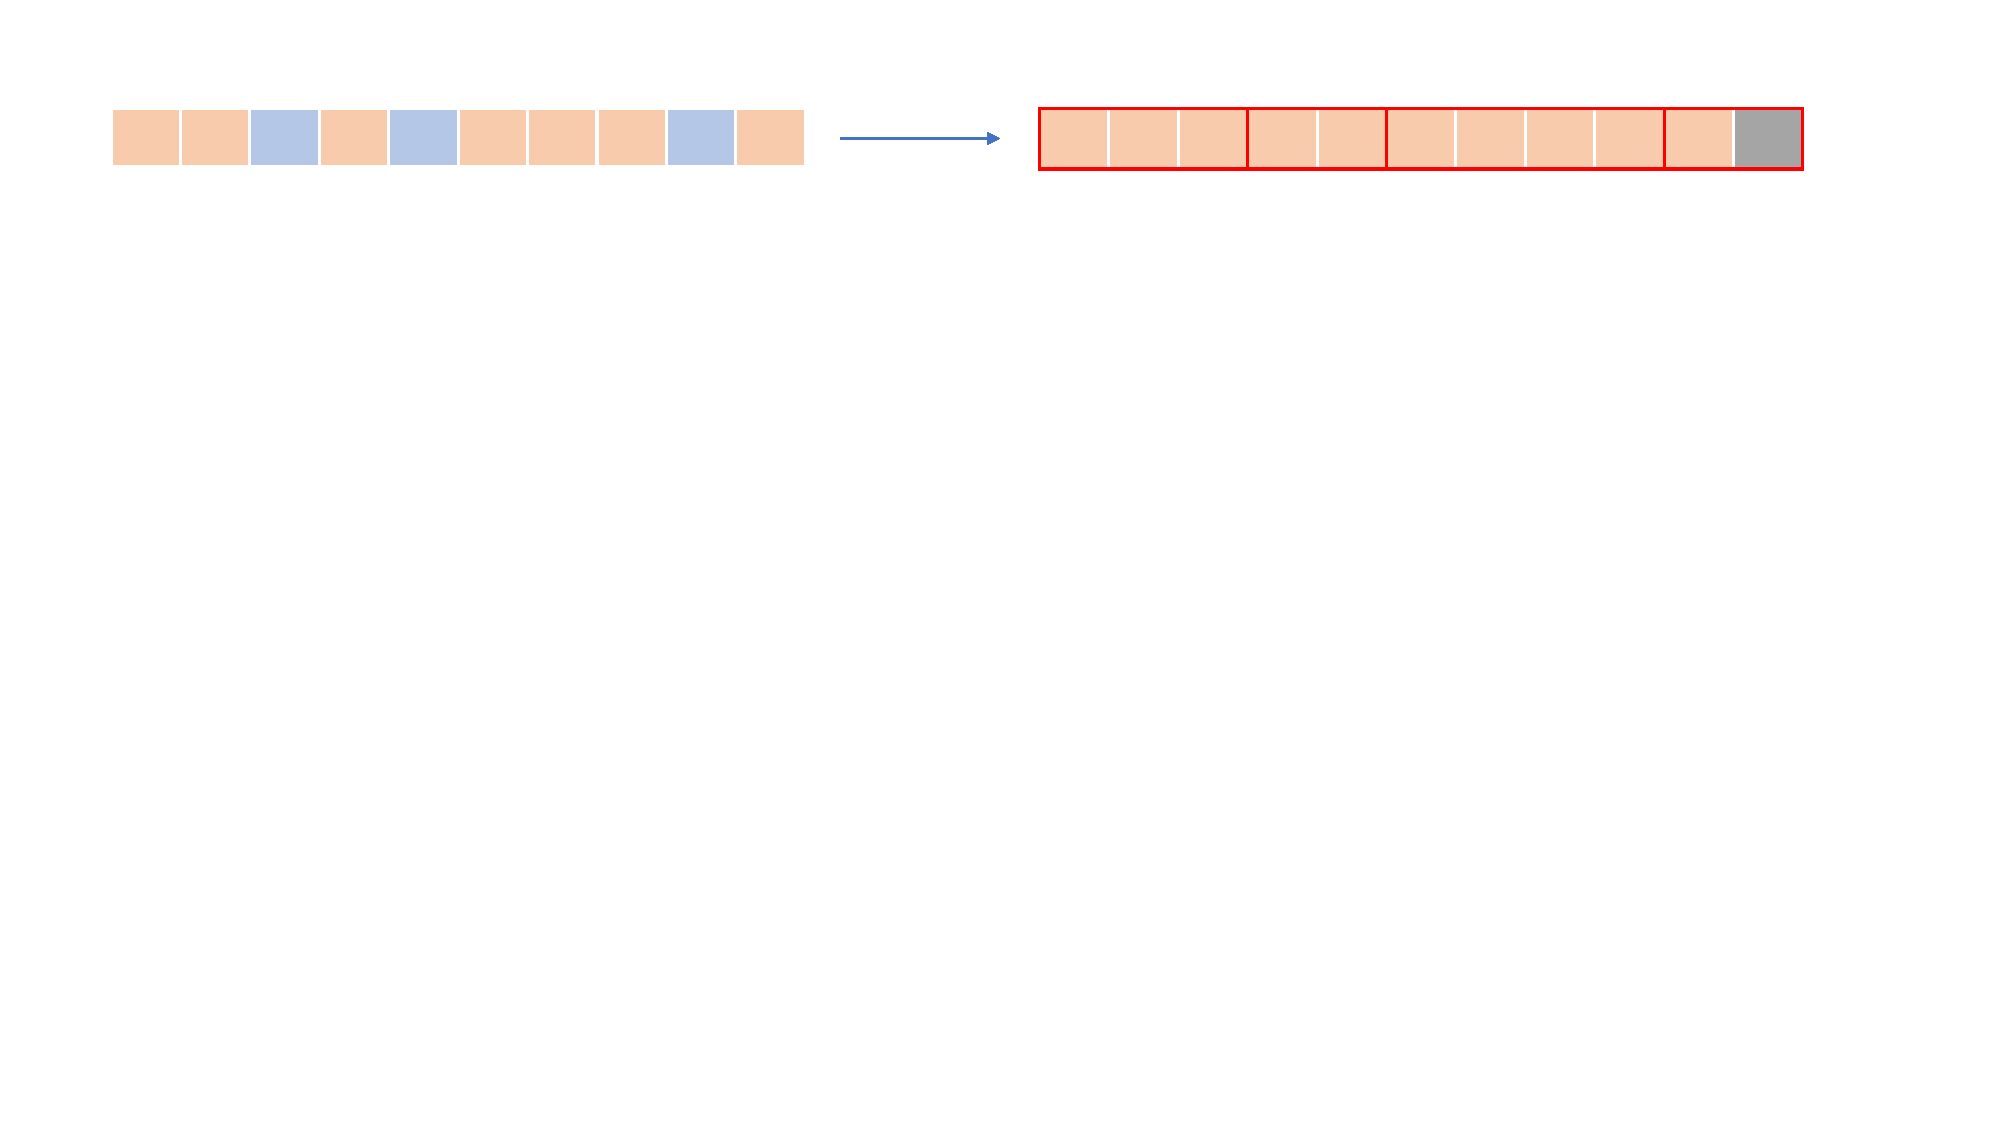
\includegraphics[width = 0.8\textwidth]{./Figures/dummy_seat.pdf}
    \caption{Problem Conversion}
\end{figure}

The social distancing here is one seat. On the left side of the diagram, the blue squares represent the empty seats required for social distancing, while the orange squares represent the seats occupied by groups. On the right side, we have added one dummy seat at the end of each row. The orange squares surrounded by the red line represent the seats taken by groups in this row, which includes two groups of 1, one group of 2, and one group of 3.

By incorporating the additional seat and designating certain seats for social distancing, we can integrate social distancing measures into the seat planning problem.


Now, we analyse the effect of introducing social distancing for each row. At first, we consider the types of pattern, which refers to the seat planning for each row. For each pattern $k$, we use $\alpha_k, \beta_k$ to indicate the number of groups and the left seats, respectively. Denote by $l(k) = \alpha_k \delta + \beta_k - \delta$ the loss for pattern $k$. The loss represents the number of people lost compared to the situation without social distancing.

Let $I_1$ be the set of patterns with the minimal loss. Then we call the patterns from $I_1$ are the largest. Similarly, the patterns from $I_2$ are the second largest, so forth and so on. The patterns with zero left seat are called full patterns. Suppose there are $n$ groups in a row, for ease of brevity, we use a descending form $P_{k} = (t_1, t_2, \ldots, t_n)$ to denote pattern $k$, where $t_h$ is the new group size, $h = 1,\ldots, n$.


\begin{example}
  Suppose the social distancing is one seat and there are four types of groups, then the new sizes of groups are $2, 3, 4, 5$, respectively. The length of one row is $L = 21$. Then these patterns, $(5, 5, 5, 5), (5, 4, 4, 4, 4),(5, 5, 5, 3, 3)$, belong to $I_1$. 
\end{example}

% To represent a pattern with a fixed length of form, we can use a $(M+1)-$dimensional vector with $M$ group types. The aggregated form can be expressed as $[n_0, n_1, \ldots, n_M]$, where $n_i$ is the number of $i$-th group type, $i \in \mathcal{M}$. $n_0$ is the number of left seat, its value can only be $0, 1$ because two or more left seats will be assigned to groups. Thus the pattern, $[1, 0, 0, 0, 4]$, is not full because there is one left seat.

We can use the following greedy way to generate the largest pattern. Select the maximal group size, $n_M$, as many as possible and the left space is assigned to the group with the corresponding size. Let $L = n_M \cdot q + r, 0 \leq r < n_M$, where $q$ is the quotient representing the number of times $n_M$ selected and $r$ is the remainder representing the number of remaining seats. The loss of the largest pattern is $q \delta -\delta + f(r)$, where $f(r)=0$ if $r> \delta$, and $f(r)=r$ if $r \leq \delta$.

% when given the length of a row, $L$, and the new size of the largest group allowed, $n_M$.

% \begin{lem}
% The seat assignment made up of the largest patterns is optimal.
% \end{lem}

% This lemma holds because we cannot find a better solution occupying more seats. When the demand can meet that the largest patterns can be generated in all rows, an optimal seat assignment can be obtained.

\begin{prop}
For a seat layout, $\{S_1, S_2, \ldots, S_{N}\}$, the minimal total loss is $\sum_{j} (\lfloor \frac{S_j+\delta}{n_{M}} \rfloor -\delta + f((S_j +\delta) \mod n_{M}))$. The maximal number of people assigned is $\sum_{j} (S_j - \lfloor \frac{S_j+\delta}{n_{M}} \rfloor + \delta - f((S_j +\delta)\mod n_{M}))$.
\end{prop}

\subsection{Dynamic Seat Assignment with Social Distancing}\label{sec_dynamic}
Consider a scenario in which groups arrive dynamically and a decision-maker must determine whether to accept or reject each group and assign them to empty seats in some row while ensuring that the social distancing constraint is met. Once seats are confirmed and assigned to a group, they cannot be changed. To keep track of the remaining capacity of rows, we use a vector $\mathbf{L} = (L_1^r, L_2^r, \ldots, L_N^r)$, where $L_j^r$ represents the number of remaining seats in row $j$. There are $T$ periods, and exactly one group request for each period. We assume that arrivals of different group types are independent, and the arrival probability of group type $i$ in each period is $p_i$. Let $V_t(\mathbf{L})$ denote the maximal expected value at period $t$ with the capacity of rows.

In every period, a decision is made on whether to accept or reject a group and which row to assign the group to. Let $u_{i,j}$ denote the decision, where $u_{i,j}(t) = 1$ if we accept a group type $i$ in row $j$ at period $t$, and $u(t) = 0$ otherwise.

The dynamic programming formulation for this problem is

$$V_{t}(\mathbf{L}) = \max_{u \in U(\mathbf{L})}\{ \sum_{i=1}^{M} p_i ( \sum_{j=1}^{N} i u_{i,j} + V_{t+1}(\mathbf{L}- \sum_{j=1}^{N} n_i u_{i,j}\mathbf{e}_j^{\top} ))\}, \mathbf{L} \geq 0, V_{T+1}(\mathbf{L}) =0, \forall \mathbf{L}$$

The decision set $U(\mathbf{L}) = \{u_{i,j} \in\{0,1\}, \forall i,j| \sum_{j=1}^{N} u_{i,j} \leq 1, \forall i, n_{i}u_{i,j}\mathbf{e}_j^{\top} \leq \mathbf{L}, \forall i,j \}$ and $\mathbf{e}_j$ is the N-dimensional unit row vector with $j$-th element being 1.

The compact form can be written as:
$$V_{t}(\mathbf{L}) = \mathbb{E}_{i \sim p}\left[\max_{\substack{j \in \mathcal{N}: \\ L_j \geqslant n_{i}}}\left\{V_{t+1}\left(\mathbf{L}- n_{i}\mathbf{e}_j^{\top} \right)+ i, V_{t+1}(\mathbf{L})\right\}\right]$$

Initially, we have $\mathbf{L}_{T} = (L_1, L_2, \ldots, L_{N})$. As we can observe, the dynamic programming algorithm has to make a decision on which row to assign group type $i$. This leads to the curse of dimensionality due to the numerous seat planning combinations. To avoid this complexity, we propose an approach that directly targets the final seat planning and then formulate a policy for assigning groups. To obtain the final seat planning firstly, we develop the scenario-based stochastic programming.

% The number of all seats in each row is called the length of the row.


% Specifically, we define the concept of target seating plans deemed satisfactory. In making the dynamic seating plan, we will try to maintain the possibility of achieving one of the target seating plans as much as possible.


% !TEX root = ./sum1.tex
% \section{Stochastic Demands Situation}

\section{Scenario-based Stochastic Programming}
This section focuses on seat planning in scenarios with varying demand. We begin by introducing a scenario-based stochastic programming formulation. However, due to its time-consuming nature, we transform it into a two-stage problem and implement benders decomposition to obtain the optimal linear solution. Using this solution, we generate a feasible seat planning.

\subsection{Formulation}
Now suppose the demand of groups is stochastic, the stochastic information can be obtained from scenarios through historical data. Use $\omega$ to index the different scenarios, each scenario $\omega \in \Omega$. A particular realization of the demand vector can be represented as $\mathbf{d}_\omega = (d_{1\omega},d_{2\omega},\ldots,d_{M,\omega})^{\intercal}$. Let $p_{\omega}$ denote the probability of any scenario $\omega$, which we assume to be positive. To maximize the expected value of people over all the scenarios, we propose a scenario-based stochastic programming.

Consider the decision makers who give the seat planning based on the scenarios then assign the groups to seats according to the realized true demand. 

The seat planning can be denoted by decision variables $\mathbf{x}\in \mathbb{Z}_{+}^{M \times N}$. Let $x_{i,j}$ stand for the number of group type $i$ in row $j$. The supply for group type $i$ can be represented by $\sum_{j=1}^N x_{ij}$.
Regarding the nature of the obtained information, we assume that there are $S = |\Omega|$ possible scenarios. There is a scenario-dependent decision variable, $\mathbf{y}$, to be chosen. It includes two vectors of decisions, $\mathbf{y}^{+} \in \mathbb{Z}_{+}^{M \times S}$ and $\mathbf{y}^{-} \in \mathbb{Z}_{+}^{M \times S}$. Each component of $\mathbf{y}^{+}$, $y_{i}^{\omega(+)}$, represents the number of surplus seats for group type $i$. Similarly, $y_{i}^{\omega(-)}$ represents the number of inadequate seats for group type $i$.
Considering that the group can take the seats planned for the larger group type, we assume that the surplus seats for group type $i$ can be occupied by smaller group type $j<i$ in the descending order of the group size. That is, for any $\omega$, $i \leq M-1$, $y_{i \omega}^{+}=\left(\sum_{j=1}^N x_{ij}- d_{i \omega} + y_{i+1, \omega}^{+}\right)^{+}$ and $y_{i \omega}^{-}=\left(d_{i \omega}- \sum_{j=1}^N x_{ij} - y_{i+1, \omega}^{+} \right)^{+}$, where $(x)^{+}$ equals $x$ if $x>0$, $0$ otherwise. Specially, for the largest group type $M$, we have $y_{M \omega}^{+} = (\sum_{j=1}^N x_{ij} - d_{i \omega})^{+}$, $y_{M \omega}^{-} = (d_{i \omega}- \sum_{j=1}^N x_{ij})^{+}$.

% These variables are scenario-independent and 

% Because the demand is unknown when the seat assignment is planned, there is no way to expect that the supply in the first stage can meet the demand exactly. Fortunately, we can find some remedies in practice, for example, seats of 5 can be assigned to a group of 4 with one empty seat as social distancing. However, the decision maker will confront seats shortage or excess without these measures. Therefore, to deal with possible demands, the wait-and-see measures (called recourses) should be considered in planning seat assignment.

% If no group of 1 comes in the future, this wait-and-see measure may leave two empty seats. 

% and that the true demand is only revealed after $\mathbf{x}$ is chosen.

% which is positive when the supply is larger than the actual demand, zero otherwise.
% which is positive when the supply is less than the actual demand and zero otherwise.

% which include the number of holding groups, $y_{i \omega}^{+}$, positive when the supply overestimates the actual demand and the number of short groups, $y_{i \omega}^{-}$, positive when the supply understimates the actual demand for group type $i$ in scenario $\omega$.

% The assignment will be determined before the realization of the random demand, here-and-now policy.

Then we have the deterministic equivalent form(DEF) of the scenario-based stochastic programming:
    \begin{align}
    (DEF) \quad \max \quad & E_{\omega}\left[\sum_{i=1}^{M-1} (n_i-\delta) (\sum_{j= 1}^{N} x_{ij} + y_{i+1,\omega}^{+} - y_{i \omega}^{+}) + (n_{M}-\delta) (\sum_{j= 1}^{N} x_{Mj} - y_{M \omega}^{+})\right] \\
    \text {s.t.} \quad & \sum_{j= 1}^{N} x_{ij}-y_{i \omega}^{+}+
    y_{i+1, \omega}^{+} + y_{i \omega}^{-}=d_{i \omega}, \quad i = 1,\ldots, M-1, \omega \in \Omega \label{DEF_constr1} \\
    & \sum_{j= 1}^{N} x_{ij} -y_{i \omega}^{+}+y_{i \omega}^{-}=d_{i \omega}, \quad i = M, \omega \in \Omega \label{DEF_constr2}\\
    & \sum_{i=1}^{M} n_{i} x_{ij} \leq L_j, j \in \mathcal{N}  \label{DEF_constr3} \\
    & y_{i \omega}^{+}, y_{i \omega}^{-} \in \mathbb{Z}_{+}, \quad i \in \mathcal{M}, \omega \in \Omega \\
    & x_{ij} \in \mathbb{Z}_{+}, \quad i \in \mathcal{M}, j \in \mathcal{N}.
    \end{align}

The objective function contains two parts, the number of the largest group type that can be accommodated is $\sum_{j= 1}^{N} x_{Mj} - y_{M \omega}^{+}$. The number of group type $i$ that can be accommodated is $\sum_{j= 1}^{N} x_{ij} + y_{i+1,\omega}^{+} - y_{i \omega}^{+}$. $E_{\omega}$ is the expectation with respect to the scenario set.

By reformulating the objective function, we have

\begin{align*}
  & E_{\omega}\left[\sum_{i=1}^{M-1} (n_i-\delta) (\sum_{j= 1}^{N} x_{ij} + y_{i+1,\omega}^{+} - y_{i \omega}^{+}) + (n_M-\delta) (\sum_{j= 1}^{N} x_{Mj} - y_{M \omega}^{+})\right] \\
  =& \sum_{j =1}^{N} \sum_{i=1}^M (n_i- \delta) x_{ij} - \sum_{\omega =1}^{S} p_{\omega} \left(\sum_{i=1}^{M}(n_i- \delta)y_{i \omega}^{+} - \sum_{i=1}^{M-1}(n_i-\delta)y_{i+1, \omega}^{+}\right) \\
  =& \sum_{j =1}^{N} \sum_{i=1}^M i \cdot x_{ij} - \sum_{\omega =1}^{S} p_{\omega} \sum_{i = 1}^{M} y_{i \omega}^{+}
\end{align*}

% Plug in $s_i = i+1$, the objective function is $\sum_{j =1}^{N} \sum_{i=1}^m i x_{ij} - \sum_{\omega =1}^{S} p_{\omega} \sum_{i=1}^{m} y_{i \omega}^{+}$.

The last equality holds because of $n_i- \delta = i, i \in \mathcal{M}$. 

\begin{remark}
For any $i, \omega$, at most one of $y_{i \omega}^{+}$ and $y_{i \omega}^{-}$ can be positive. 
Suppose there exist $i_0$ and $\omega_0$ such that $y_{i_0 \omega_0}^{+}$ and $y_{i_0 \omega_0}^{-}$ are positive. Substracting $\min\{y_{i_0, \omega_0}^{+}, y_{i_0, \omega_0}^{-}\}$ from these two values will still satisfy constraints \eqref{DEF_constr1} and \eqref{DEF_constr2} but increase the objective value when $p_{\omega_0}$ is positive. Thus, at most one of $y_{i \omega}^{+}$ and $y_{i \omega}^{-}$ can be positive. 
\end{remark}

Let $\mathbf{n} = (n_1, \ldots, n_M)$, $\mathbf{L} = (L_1, \ldots, L_N)$ where $s_i$ is the size of seats taken by group type $i$ and $L_j$ is the length of row $j$ as we defined above. Then the constraint \eqref{DEF_constr3} can be expressed as $\mathbf{n} \mathbf{x} \leq \mathbf{L}$.

The linear constraints associated with scenarios, i.e., constraints \eqref{DEF_constr1} and \eqref{DEF_constr2}, can be written in a matrix form as
\[\mathbf{x} \mathbf{1} + \mathbf{V} \mathbf{y}_\omega = \mathbf{d}_\omega, \omega\in \Omega,\]

where $\mathbf{1}$ is a column vector of size $N$ with all 1s, $\mathbf{V} = [\mathbf{W}, ~\mathbf{I}]$.

$$
\mathbf{W}=\left[\begin{array}{ccccc}
-1 & 1 & \ldots & & 0 \\
& \ddots & \ddots & & \vdots \\
& & & & 1 \\
0 & & & & -1
\end{array}\right]_{M \times M}
$$

and $\mathbf{I}$ is the identity matrix. For each scenario $\omega \in \Omega$,
$$
\mathbf{y}_{\omega}=\left[\begin{array}{l}
\mathbf{y}_{\omega}^{+} \\
\mathbf{y}_{\omega}^{-}
\end{array}\right], \mathbf{y}_{\omega}^{+}=\left[\begin{array}{lllll}y_{1 \omega}^{+} & y_{2 \omega}^{+} & \cdots & y_{M \omega}^{+}\end{array}\right]^{\intercal}, \mathbf{y}_{\omega}^{-}=\left[\begin{array}{llll}y_{1 \omega}^{-} & y_{2 \omega}^{-} & \cdots & y_{M \omega}^{-}\end{array}\right]^{\intercal}.
$$

As we can find, this deterministic equivalent form is a large-scale problem even if the number of possible scenarios $\Omega$ is moderate. However, the structured constraints allow us to simplify the problem by applying Benders decomposition approach. Before using this approach, let us write this problem in the form of the two-stage stochastic programming.

Let $\mathbf{c}^{\intercal}\mathbf{x} = \sum_{j =1}^{N} \sum_{i=1}^M i \cdot x_{ij}$, $\mathbf{f}^{\intercal}\mathbf{y}_{\omega} = -\sum_{i=1}^{M} y_{i \omega}^{+}$. Then the DEF formulation can be expressed as below,

\begin{equation}\label{BD_master}
  \begin{aligned}
\max \quad & \mathbf{c}^{\intercal} \mathbf{x}+ z(\mathbf{x}) \\
\text {s.t.} \quad & \mathbf{n} \mathbf{x} \leq \mathbf{L} \\
& \mathbf{x} \in \mathbb{Z}_{+}^{M \times N},
\end{aligned}
\end{equation}

where $z(\mathbf{x})$ is the recourse function defined as 

$$z(\mathbf{x}) := E(z_{\omega}(\mathbf{x})) = \sum_{\omega \in \Omega} p_{\omega} z_{\omega}(\mathbf{x}),$$ and for each scenario $\omega \in \Omega$, 

\begin{equation}\label{BD_sub}
  \begin{aligned}
    z_{\omega}(\mathbf{x}) := \max \quad & \mathbf{f}^{\intercal} \mathbf{y}_{\omega} \\
    \text {s.t.} \quad & \mathbf{x} \mathbf{1} + \mathbf{V} \mathbf{y}_{\omega} = \mathbf{d}_{\omega} \\
     & \mathbf{y}_{\omega} \geq 0.
  \end{aligned}
  \end{equation}

% The objective function of problem \eqref{sto_form} can be expressed as $c{'}\mathbf{x} + \sum_{\omega} p_{\omega}f{'}y_{\omega}$. 
Problem \eqref{BD_sub} stands for the second-stage problem and $z_{\omega}(\mathbf{x})$ is the optimal value of problem \eqref{BD_sub}, together with the convention $z_{\omega}(\mathbf{x}) = \infty$ if the problem is infeasible.

Solving the above problem directly can be challenging, so we first obtain the optimal solution to the relaxation of problem \eqref{BD_master}. From this solution, we generate a seat planning.

\subsection{Solve the Scenario-based Two-stage Problem}\label{solve_by_benders}
At first, we generate a closed-form solution to the second-stage problem in section \ref{second_stage}. Then we obtain the solution to the linear relaxation of problem \eqref{BD_master} by the delayed constraint generation. Finally, we obtain a feasible seat planning from the linear solution.

\subsubsection{Solve the Second Stage Problem}\label{second_stage}

Consider a $\mathbf{x}$ such that $\mathbf{n x} \leq \mathbf{L}$ and $\mathbf{x} \geq 0$ and suppose that this represents the seat planning. Once $\mathbf{x}$ is fixed, the optimal decisions $\mathbf{y}_{\omega}$ can be determined by solving problem \eqref{BD_sub} for each $\omega$.

% To solve this problem, we should only consider that $\mathbf{x}$ for which $z_{\omega}(\mathbf{x})$ are all finite. 
Notice that the feasible region of the dual of problem \eqref{BD_sub} does not depend on $\mathbf{x}$. Let $\bm{\alpha}$ be the vector of dual variable. For each $\omega$, we can form its dual problem, which is 

\begin{equation}\label{BD_sub_dual}
  \begin{aligned}
    \min \quad & \bm{\alpha}^{\intercal} (\mathbf{d}_{\omega}- \mathbf{x} \mathbf{1}) \\
    \text {s.t.} \quad & \bm{\alpha}^{\intercal} \mathbf{V} \geq \mathbf{f}^{\intercal}
  \end{aligned}
  \end{equation}

Let $\mathbb{P} = \{\bm{\alpha} \in \mathbb{R}^{M}|\bm{\alpha}^{\intercal} \mathbf{V} \geq \mathbf{f}^{\intercal}\}$. 
We assume that $\mathbb{P}$ is nonempty and has at least one extreme point. Then, either the dual problem \eqref{BD_sub_dual} has an optimal solution and $z_{\omega}(\mathbf{x})$ is finite, or the primal problem \eqref{BD_sub} is infeasible and $z_{\omega}(\mathbf{x}) = \infty$.  

Let $\mathcal{O}$ be the set of all extreme points of $\mathbb{P}$ and $\mathcal{F}$ be the set of all extreme rays of $\mathbb{P}$. Then $z_{\omega} > -\infty$ if and only if $\bm{\alpha}^{\intercal}(\mathbf{d}_{\omega}- \mathbf{x} \mathbf{1}) \geq 0, \bm{\alpha} \in \mathcal{F}$, which stands for the feasibility cut.

\begin{lem}\label{feasible_region}
  The feasible region of problem \eqref{BD_sub_dual}, $\mathbb{P}$, is bounded. In addition, all the extreme points of $\mathbb{P}$ are integral.
\end{lem}

\begin{pf}[Proof of lemma \ref{feasible_region}]
Notice that $\mathbf{f}^{\intercal} = [-\mathbf{1},~\mathbf{0}], V =[W,~I]$, $W$ is a totally unimodular matrix. Then, we have $\bm{\alpha}^{\intercal}W \geq -\mathbf{1}, \bm{\alpha}^{\intercal} I \geq \mathbf{0}$. Thus, the feasible region is bounded. 
Furthermore, let $\alpha_0 = 0$, then we have $0 \leq \alpha_i \leq \alpha_{i-1} +1$, $i \in \mathcal{M}$, so the extreme points are all integral.
\qed
\end{pf}

Because the feasible region is bounded, then feasibility cuts are not needed. Let $z_{\omega}$ be the lower bound of $z_{\omega}(x)$ such that $\bm{\alpha}^{\intercal}(\mathbf{d}_{\omega}- \mathbf{x} \mathbf{1}) \geq z_{\omega}, \bm{\alpha} \in \mathcal{O}$, which is the optimality cut.

\begin{corollary}
  Only the optimality cuts, $\alpha^{\intercal}(\mathbf{d}_{\omega}- \mathbf{x} \mathbf{1}) \geq z_{\omega}$, will be included in the decomposition approach.
\end{corollary}

\begin{corollary}
The optimal value of the problem \eqref{BD_sub}, $z_{\omega}(x)$, is finite and will be attained at extreme points of the set $P$. Thus, we have $z_{\omega}(x) = \min_{\bm{\alpha} \in \mathcal{O}} \bm{\alpha}^{\intercal}(\mathbf{d}_{\omega}- \mathbf{x} \mathbf{1})$. 
\end{corollary}


When we are given $\mathbf{x}^{*}$, the demand that can be satisfied by the assignment is $\mathbf{x}^{*} \mathbf{1} = \mathbf{d}_0 = (d_{1,0},\ldots,d_{M,0})^{\intercal}$.
Then plug them in the subproblem \eqref{BD_sub}, we can obtain the value of $y_{i \omega}$ recursively:
\begin{equation}\label{y_recursively}
\begin{aligned}
  & y_{M \omega}^{-}=\left(d_{M \omega}-d_{M 0}\right)^{+} \\
  & y_{M \omega}^{+}=\left(d_{M 0}-d_{M \omega}\right)^{+} \\
  & y_{i \omega}^{-}=\left(d_{i \omega}-d_{i 0} - y_{i+1, \omega}^{+} \right)^{+}, i =1,\ldots, M-1 \\
  & y_{i \omega}^{+}=\left(d_{i 0}- d_{i \omega} + y_{i+1, \omega}^{+}\right)^{+}, i =1,\ldots, M-1
\end{aligned}
\end{equation}

The optimal value for scenario $\omega$ can be obtained by $\mathbf{f}^{\intercal} y_{\omega}$, then we need to find the dual optimal solution.


\begin{thm}\label{optimal_sol_sub_dual}
  The optimal solutions to problem \eqref{BD_sub_dual} are given by 
\begin{equation}\label{BD_sub_simplified}
  \begin{aligned}
    & \alpha_{i} = 0, i \in \mathcal{M} \quad \text{if}~  y_{i \omega}^{-} > 0,  y_{i \omega}^{+} = 0   \\
    & \alpha_{i} = \alpha_{i-1}+1, i \in \mathcal{M} \quad \text{if}~ y_{i \omega}^{+} > 0,  y_{i \omega}^{-} = 0 \\
    & \alpha_{i} = 0, i =1,\ldots, M-1 \quad \text{if}~ y_{i \omega}^{-} = y_{i \omega}^{+} = 0, y_{i+1, \omega}^{+}> 0 \\
    & 0 \leq \alpha_{i} \leq \alpha_{i-1}+1, i =1,\ldots, M-1 \quad \text{if}~ y_{i \omega}^{-} = y_{i \omega}^{+} = 0, y_{i+1, \omega}^{+}= 0 \\
    & 0 \leq \alpha_{i} \leq \alpha_{i-1}+1, i = M \quad \text{if}~ y_{i \omega}^{-} = y_{i \omega}^{+} = 0
  \end{aligned}
\end{equation}
\end{thm}

\begin{pf}[Proof of Theorem \ref{optimal_sol_sub_dual}]
According to the complementary slackness property, we can obtain the following equations
\begin{align*}
  & \alpha_{i} (d_{i0} - d_{i \omega} - y_{i \omega}^{+} + y_{i+1, \omega}^{+} + y_{i \omega}^{-}) = 0, i =1,\ldots, M-1 \\
  & \alpha_{i} (d_{i0} - d_{i \omega} - y_{i \omega}^{+}+ y_{i \omega}^{-}) = 0, i = M \\
  & y_{i \omega}^{+}(\alpha_{i} - \alpha_{i-1}-1) = 0, i =1,\ldots, M \\
  & y_{i \omega}^{-} \alpha_{i} = 0, i =1,\ldots, M.
\end{align*}

When $y_{i \omega}^{-} >0$, we have $\alpha_{i} =0$; when $y_{i \omega}^{+} >0$, we have $\alpha_{i} = \alpha_{i-1} +1$.
Let $\Delta d = d_{\omega} - d_0$, then the elements of $\Delta d$ will be a negative integer, positive integer and zero.
When $y_{i \omega}^{+} = y_{i \omega}^{-} = 0$, if $i = M$, $\Delta d_{M} =0$, the value of objective function associated with $\alpha_{M}$ is always $0$, thus we have $0 \leq \alpha_{M} \leq \alpha_{M-1}+1$; if $i < M$, we have $y_{i+1, \omega}^{+} = \Delta d_{i} \geq 0$. If $y_{i+1, \omega}^{+} > 0$, the objective function associated with $\alpha_i$ is $\alpha_{i} \Delta d_{i} = \alpha_{i} y_{i+1, \omega}^{+}$, thus to minimize the objective value, we have $\alpha_i =0$; if $y_{i+1, \omega}^{+} = 0$, we have $0 \leq \alpha_{i} \leq \alpha_{i-1} +1$.
\qed
\end{pf}

% \begin{remark}
% During the calculation, we choose the optimal solution $\alpha_{i} = \alpha_{i-1} +1$ when $0 \leq \alpha_{i} \leq \alpha_{i-1} +1$.
% \end{remark}

We can use the forward method, calculating from $\alpha_{1 \omega}$ to $\alpha_{M \omega}$, to obtain the value of $\alpha_{\omega}$ instead of solving the original large-scale linear programming.

\subsubsection{Delayed Constraint Generation}\label{bender_stage}
Benders decomposition works with only a subset of those exponentially many constraints and adds more constraints iteratively until the optimal solution of Benders Master Problem(BMP) is attained. This procedure is known as delayed constraint generation.

% Restricted Benders master problem:
Use the characterization of $z_{\omega}(x)$ in the problem \eqref{BD_master} and take into account the optimality cuts, we can conclude the BMP will have the form:

\begin{equation}\label{BD_master2}
  \begin{aligned}
    \max \quad & \mathbf{c}^{\intercal} \mathbf{x} + \sum_{\omega \in \Omega} p_{\omega} z_{\omega} \\
    \text {s.t.} \quad & \mathbf{n} \mathbf{x} \leq \mathbf{L} \\
    & \bm{\alpha}^{\intercal}(\mathbf{d}_{\omega}- \mathbf{x} \mathbf{1}) \geq z_{\omega}, \bm{\alpha} \in \mathcal{O}, \forall \omega \\
     & \mathbf{x} \geq 0, z_{\omega} ~\text{is free}
  \end{aligned}
\end{equation}

When substituting $\mathcal{O}$ with its subset, $\mathcal{O}^{t}$, the problem \eqref{BD_master2} becomes the Restricted Benders Master Problem(RBMP). 

To determine the initial $\mathcal{O}^{t}$, we have the following lemma.

\begin{lem}\label{one_ep_feasible}
RBMP is always bounded with at least any one optimality cut for each scenario.
\end{lem}

\begin{pf}[Proof of lemma \ref{one_ep_feasible}]
  Suppose we have one extreme point $\bm{\alpha}_{\omega}^{0}$ for each scenario. Then we have the following problem.
  \begin{equation}\label{lemma_eq}
    \begin{aligned}
      \max \quad & \mathbf{c}^{\intercal} \mathbf{x} + \sum_{\omega \in \Omega} p_{\omega} z_{\omega} \\
      \text {s.t.} \quad & \mathbf{n} \mathbf{x} \leq \mathbf{L} \\
      & (\bm{\alpha}_{\omega}^{0})^{\intercal}\mathbf{d}_{\omega} \geq (\bm{\alpha}_{\omega}^{0})^{\intercal} \mathbf{x} \mathbf{1} + z_{\omega}, \forall \omega \\
       & \mathbf{x} \geq 0
    \end{aligned}
  \end{equation}
  Problem \eqref{lemma_eq} reaches its maximum when $(\bm{\alpha}_{\omega}^{0})^{\intercal}\mathbf{d}_{\omega} = (\bm{\alpha}_{\omega}^{0})^{\intercal} \mathbf{x} \mathbf{1} + z_{\omega}, \forall \omega$. Substitute $z_{\omega}$ with these equations, we have 
  \begin{equation}\label{lemma_eq2}
    \begin{aligned}
      \max \quad & \mathbf{c}^{\intercal} \mathbf{x} - \sum_{\omega}p_{\omega}(\bm{\alpha}_{\omega}^{0})^{\intercal} \mathbf{x} \mathbf{1} + \sum_{\omega} p_{\omega} (\bm{\alpha}_{\omega}^{0})^{\intercal} \mathbf{d}_{\omega} \\
      \text {s.t.} \quad & \mathbf{n} \mathbf{x} \leq \mathbf{L} \\
      & \mathbf{x} \geq 0
    \end{aligned}
  \end{equation}
  Notice that $\mathbf{x}$ is bounded by $\mathbf{L}$, then the problem \eqref{lemma_eq} is bounded. Adding more optimality cuts will not make the optimal value larger. Thus, RBMP is bounded. 
  \qed
\end{pf}

Given the initial $\mathcal{O}^{t}$, we can have the solution $\mathbf{x}_{0}$ and $\mathbf{z}^{0} =(z^{0}_1,\ldots, z^{0}_S)$. Then $c^{\intercal} \mathbf{x}_0 + \sum_{\omega \in \Omega} p_{\omega} z_{\omega}^{0}$ is an upper bound of problem \eqref{BD_master2}. 


When $\mathbf{x}_0$ is given, the optimal solution, $\bm{\alpha}_{\omega}^{1}$, to problem \eqref{BD_sub_dual} can be obtained according to Theorem \ref{optimal_sol_sub_dual}. $z_{\omega}^{(0)} = \bm{\alpha}_{\omega}^{1}(d_{\omega} - \mathbf{x}_0 \mathbf{1})$ and $(\mathbf{x}_0, \mathbf{z}^{(0)})$ is a feasible solution to problem \eqref{BD_master2} because it satisfies all the constraints. Thus, $\mathbf{c}^{\intercal} \mathbf{x}_0 + \sum_{\omega \in \Omega} p_{\omega} z_{\omega}^{(0)}$ is a lower bound of problem \eqref{BD_master2}.

If for every scenario $\omega$, the optimal value of the corresponding problem \eqref{BD_sub_dual} is larger than or equal to $z_{\omega}^{0}$, all contraints are satisfied, we have an optimal solution, $(\mathbf{x}_{0}, \mathbf{z}_{\omega}^{0})$, to the BMP. Otherwise, add one new constraint, $(\bm{\alpha}_{\omega}^{1})^{\intercal}(\mathbf{d}_{\omega}- \mathbf{x} \mathbf{1}) \geq z_{\omega}$, to RBMP.

% $z_{\omega}^{(0)} = \alpha_{\omega}^{*}(d_{\omega} - \mathbf{x}_0 \mathbf{1})$ will give a minimal upper bound of $z_{\omega}$, thus all the left constraints associated with other extreme points are redundant.when the extreme points are $\alpha_{\omega}$.

% The problem \eqref{lemma_eq} associated with $\alpha_{\omega}$ will give an optimal solution $(x_1, z_{\omega}^{1})$. (Upper bound)


The steps of the algorithm are described as below,

\begin{algorithm}[H]\label{cut_algo}
  \caption{The benders decomposition algorithm}
    \begin{description}
    \item[Step 1.] Solve LP \eqref{lemma_eq} with all $\alpha_{\omega}^0 = \mathbf{0}$ for each scenario. Then, obtain the solution $(\mathbf{x}_0, \mathbf{z}^{0})$.
    \item[Step 2.] Set the upper bound $UB = c^{\intercal} \mathbf{x}_0 + \sum_{\omega \in \Omega} p_{\omega} z_{\omega}^{0}$.
    \item[Step 3.] For $x_0$, we can obtain $\alpha_{\omega}^{1}$ and $z_{\omega}^{(0)}$ for each scenario, set the lower bound $LB = c^{\intercal} x_0 + \sum_{\omega \in \Omega} p_{\omega} z_{\omega}^{(0)}$.
    \item[Step 4.] For each $\omega$, if $(\alpha_{\omega}^{1})^{\intercal}(\mathbf{d}_{\omega}- \mathbf{x}_0 \mathbf{1}) < z_{\omega}^{0}$, add one new constraint, $(\alpha_{\omega}^{1})^{\intercal}(\mathbf{d}_{\omega}- \mathbf{x} \mathbf{1}) \geq z_{\omega}$, to RBMP.
    \item[Step 5.] Solve the updated RBMP, obtain a new solution $(x_1, z^{1})$ and update UB.
    \item[Step 6.] Repeat step 3 until $UB - LB < \epsilon$.(In our case, UB converges.)
   \end{description}
  \end{algorithm}

\begin{remark}
From the Lemma \ref{one_ep_feasible}, we can set $\bm{\alpha}_{\omega}^0 = \mathbf{0}$ initially in {\bf Step 1}.
\end{remark}

\begin{remark}
Notice that only contraints are added in each iteration, thus $LB$ and $UB$ are both monotone. Then we can use $UB - LB < \epsilon$ to terminate the algorithm in {\bf Step 6}.
\end{remark}

After the algorithm terminates, we obtain the optimal $\mathbf{x}^{*}$. The demand that can be satisfied by the arrangement is $\mathbf{x}^{*} \mathbf{1} = \mathbf{d}_0 = (d_{1,0},\ldots,d_{M,0})$.
Then we can obtain the value of $\mathbf{y}_{\omega}$ from equation \eqref{y_recursively}.

% We show the results of Benders and IP in the section \ref{Bender_IP}.

\subsection{Obtain the Feasible Seat Planning}\label{seat_assignment}
The decomposition method only gives a fractional solution and the stochastic model does not provide an appropriate seat planning when the number of people in scenario demands is way smaller than the number of the seats. Thus, we change the linear solution from the decomposition method to obtain a feasible seat planning. Before that, we will discuss the deterministic model that can help to achieve the goal.

% The objective is to obtain the maximal number of people placed according to the demand scenarios. It will not provide an appropriate seat assignment when the number of people associated with scenario demands is way less than the number of available seats because there are multiple optimal solutions and the solution given by solver probably does not utilize all the empty seats.

When $|\Omega| =1$ in DEF formulation, the stochastic programming will be 

\begin{equation}\label{one_form}
  \begin{aligned}
  \max \quad & \sum_{i=1}^{M}  \sum_{j= 1}^{N} (n_i-\delta) x_{ij} - \sum_{i=1}^{M} y_{i}^{+}  \\
  \text {s.t.} \quad & \sum_{j= 1}^{N} x_{ij} - y_{i}^{+}+ y_{i+1}^{+} + y_{i}^{-} = d_{i}, \quad i = 1, \ldots, M-1, \\
  & \sum_{j= 1}^{N} x_{ij} -y_{i}^{+} + y_{i}^{-} = d_{i}, \quad i = M, \\
  & \sum_{i=1}^{M} n_{i} x_{ij} \leq L_j, j \in \mathcal{N}\\
  & y_{i}^{+}, y_{i}^{-} \in \mathbb{Z}_{+}, \quad i \in \mathcal{M} \\
  & x_{ij} \in \mathbb{Z}_{+}, \quad i \in \mathcal{M}, j \in \mathcal{N}.
  \end{aligned}
\end{equation}

To maximize the objective function, we can take $y_i^{+} = 0$. Notice that $y_{i}^{-} \geq 0$, thus the constraints $\sum_{j= 1}^{N} x_{ij} + y_{i}^{-} = d_{i}, i \in \mathcal{M}$ can be rewritten as $\sum_{j= 1}^{N} x_{ij} \leq d_{i}, i \in \mathcal{M}$, then we have

\begin{equation}\label{deter_upper}
  \begin{aligned}
  \max \quad & \sum_{i=1}^{M}  \sum_{j= 1}^{N} (n_i- \delta) x_{ij} \\
  \text {s.t.} \quad & \sum_{j= 1}^{N} x_{ij} \leq d_{i}, \quad i \in \mathcal{M}, \\
  & \sum_{i=1}^{M} n_{i} x_{ij} \leq L_j, j \in \mathcal{N} \\
  & x_{ij} \in \mathbb{Z}_{+}, \quad i \in \mathcal{M}, j \in \mathcal{N}.
  \end{aligned}
\end{equation}

Problem \eqref{deter_upper} represents the deterministic model. Demand, $d_i, i \in \mathcal{M}$ is known in advance, our goal is to accommodate as many as people possible in the fixed rows.

\begin{lem}\label{sol_relax_deter}
For the linear relaxation of problem \eqref{deter_upper}, there exists $h$ such that the optimal solutions $x_{ij}^{*} = 0$ when $i < h$; $\sum_{j} x_{ij}^{*} = d_{i}$, when $i > h$; $\sum_{j} x_{ij}^{*} = (L - \sum_{i = h+1}^{M} {d_i n_i})/ n_h$, when $i = h$.
\end{lem}

Let $\sum_{j=1}^{N} x_{ij}$ represent the supply for group type $i$. We define $\mathbf{X} = (\sum_{j=1}^{N} x_{1j},\ldots, \sum_{j=1}^{N} x_{Mj})$ as the aggregate solution to the linear relaxation of problem \eqref{deter_upper}. Furthermore, let $e_{i}$ denote the unit size of the $i$-th element of $\mathbf{X}$.

In the aggregate optimal solution, denoted as $x e_{h} + \sum_{i=h+1} ^{M} d_{i} e_{i}$, the following components are present: $x e_{h}$: This term represents the allocation of resources for group type $h$. The value of $x$ is calculated as $(L- \sum_{i = h+1}^{M} {d_i n_i})/ n_h$, indicating the remaining capacity after satisfying the demands of indices greater than $h$, divided by the unit size $n_h$. $\sum_{i=h+1} ^{M} d_{i} e_{i}$: This term accounts for the allocation of resources for group types $h+1$ to $M$. It represents the total demand for these group types, where $d_i$ denotes the demand of group type $i$, and $e_{i}$ represents the unit size of the corresponding element in $\mathbf{X}$. Together, the aggregate optimal solution combines the allocation of resources for group type $h$ with the aggregated demands for group types $h+1$ to $M$ to achieve an optimal solution to the linear relaxation of the problem.

% Suppose that each row has the same length. Then the optimal integrated solution 
% $(0,\ldots, x,d_{h+1}, \ldots, d_{m})$ has the same objective value with an integer solution. Deciding if these items can fit into a specified number of rows is the decision problem of the bin-packing problem. If the items associated with the integer solution can be put in the given number of rows, this solution is optimal; otherwise, it is not optimal. Since the bin-packing problem is NP-hard, problem \eqref{deter_upper} is also NP-hard.

% its objective is to obtain the maximal number of people served, not the optimal seat assignment. It will not provide an appropriate solution when the number of arriving people in the scenarios is way less than the number of total seats because it does not utilize all the empty seats.

Let the optimal solution to the relaxation of DEF be $x^{*}_{ij}$. Aggregate $\mathbf{x}^{*}$ to the number of each group type, ${s}_{i}^{0} =\sum_{j} x^{*}_{ij}, i \in \mathbf{M}$. Replace the vector $\mathbf{d}$ with $\mathbf{s}^{0}$, we have the following problem, 

\begin{equation}\label{deter_upper1}
  \{\max \sum_{j=1}^{N} \sum_{i=1}^{M}(n_i -\delta) x_{ij}: \sum_{i = 1}^{M} n_i x_{ij} \leq L_{j}, j \in \mathcal{N}; \sum_{j =1}^{N} x_{ij} \leq s_{i}^{0}, i \in \mathcal{M}; x_{ij} \in Z^{+} \}
\end{equation}

then solve the resulting problem \eqref{deter_upper1} to obtain the optimal solution, $\mathbf{x}^{1}$, which represents a feasible seat planning. Aggregate $\mathbf{x}^{1}$ to the number of each group type, ${s}_{i}^{1} = \sum_{j} x^{1}_{ij}, i \in \mathbf{M}$, which represents the supply for each group type.

To fully utilize the seats, we should set the supply $\mathbf{s}^{1}$ as the lower bound, then re-solve a seat planning problem. We substitute the constraint $\sum_{j =1}^{N} x_{ij} \leq d_{i}, i \in \mathcal{M}$ in problem \eqref{deter_upper} with the new constraint $\sum_{j =1}^{N} x_{ij} \geq s_{i}^{1}, i \in \mathcal{M}$.

\begin{equation}\label{deter_lower}
\{\max \sum_{j=1}^{N} \sum_{i=1}^{M}(n_i -\delta) x_{ij}: \sum_{i = 1}^{M} n_i x_{ij} \leq L_{j}, j \in \mathcal{N}; \sum_{j =1}^{N} x_{ij} \geq s_{i}^{1}, i \in \mathcal{M}; x_{ij} \in Z^{+} \}
\end{equation}

Notice that the number of unoccupied seats in the seat planning obtained from problem \eqref{deter_lower} is at most $\delta$ for each row, given any feasible supply, $\mathbf{s}^{1}$.
To maximize the utilization of seats, we should assign full or largest patterns to each row. This procedure can be described in {\bf Step 4} of the following algorithm.

\begin{algorithm}[H]
  \caption{Feasible seat planning algorithm}\label{feasible_seat}
    \begin{description}
    \item[Step 1.] Obtain the solution, $\mathbf{x}^{*}$, from stochatic linear programming by benders decomposition. Aggregate $\mathbf{x}^{*}$ to the number of each group type, ${s}_{i}^{0} =\sum_{j} x^{*}_{ij}, i \in \mathbf{M}$.

    \item[Step 2.] Solve problem \eqref{deter_upper1} to obtain the optimal solution, $\mathbf{x}^{1}$. Aggregate $\mathbf{x}^{1}$ to the number of each group type, ${s}_{i}^{1} = \sum_{j} x^{1}_{ij}, i \in \mathbf{M}$.
    
    \item[Step 3.] Obtain the optimal solution, $\mathbf{x}^{2}$, from problem \eqref{deter_lower} with supply $\mathbf{s}^{1}$. Aggregate $\mathbf{x}^{2}$ to the number of each group type, ${s}_{i}^{2} = \sum_{j} x^{2}_{ij}, i \in \mathbf{M}$.

    \item[Step 4.] Check if row $j$ is full for all $j$. When row $j^{0}$ is not full, i.e., $\sum_{i} n_{i} x_{ij} < L_{j^{0}}$, let $\beta = L_{j^{0}} - \sum_{i} n_{i} x_{ij}$. 
    Find the smallest group size in row $j^{0}$ and mark it as $i^0$. If the smallest group is exactly the largest, then the row corresponds to the largest pattern and check next row. Otherwise, reduce the number of group type $i^0$ by one and increase the number of group type $\min \{(i^0+\beta), M\}$ by one. Continue this procedure until this row is full.
   \end{description}
  \end{algorithm}

\begin{remark}
  {\bf Step 2} can give a feasible seat planning. {\bf Step 4} can give the full or largest patterns for each row.
\end{remark}

% Thus, we can obtain a feasible seat planning by solving stochastic programming once and deterministic programming twice.

% 1. Why should we don't use the subset sum problem to decompose the whole problem, it will destroy global optimality. But notice that when we arrange row by row, it may also affect the optimality.

% Many symmetry structure/ Every step we need to solve a multiple knapsack problem(difficult).

\begin{remark}
% We are able to provide an online seat planning by using our method.
For a feasible seat planning, we provide a full or largest pattern for each row. The sequence of groups within each pattern can be arranged arbitrarily, allowing for a flexible seat planning that can accommodate realistic operational constraints. Therefore, any fixed sequence of groups within each pattern can be used to construct a seat planning that meets practical needs.
\end{remark}

% !TEX root = sum1.tex
\section{Dynamic Seat Assignment Policy}\label{sec_dynamic}
% identify possible rows and assign to specific row.
In this section, we discuss the dynamic seat assignment policy, which involves making decisions on seat allocations for each group arrival based on the seat planning obtained from Section \ref{sec_seat_planning}.

When a group arrives, we first check if the corresponding supply is sufficient. If the supply is enough, we can directly accept the group and assign seats to it in the row with the corresponding supply. However, if the supply is insufficient, we need to consider alternative options. Based on our previous considerations, we know that groups can be assigned to the seats which are planned for a larger group type if the supply for their own group type is insufficient. To determine whether to use larger seats to accommodate the incoming group, we assess the potential benefits by comparing the expected values of accepting the group with larger seats and rejecting the group based on the current seat planning.
To make this decision, we identify the possible rows where the incoming group can be assigned based on the group types and seat availability. This policy is called group-type control, which helps us narrow down the option of rows for seat assignment.

If we make decisions based on the seat planning generated from SSP, when the corresponding supply is sufficient, we will accept the group, without considering that larger seats can accommodate smaller groups, which will result in rejecting too many smaller groups. Therefore, it is necessary to assess whether to accept a group with the larger seats based on the current seat planning. 

While it would be ideal to obtain the integral seat planning by solving the SSP directly, this may not be feasible due to the computational complexity and the need to calculate the value of the SSP for each potential seat assignment. The process of solving the integer programming and evaluating the stochastic programming value for each row is time-consuming, making it impractical for real-time decision-making.

In practice, to save the computation cost, we can calculate the value of the LP relaxation of the SSP. This approach provides the same value under the same scenario set, regardless of which row the group is placed in. Therefore, we only need to compare the values of accepting the group at any one row with the value of rejecting the group to make a decision.

After determining the possible rows for seat assignment using the strategies mentioned earlier, we can apply a tie-breaking rule to select a specific row. This rule helps us decide on a particular row when there are multiple options available. Next, we compare the values of the stochastic programming problem when accepting the group at the chosen row versus rejecting it. This evaluation allows us to assess the potential revenues associated with each decision. Simultaneously, after this calculation, we can generate a new seat planning according to Algorithm 3.


By combining the group-type control strategy with the evaluation of stochastic programming values, we obtain a comprehensive decision-making process within a single period. This integrated approach enables us to make informed decisions regarding the acceptance or rejection of incoming groups, as well as determine the appropriate row for their assignment when acceptance is the chosen option. By considering both computation time savings and potential revenues, we can optimize the overall performance of the seat assignment process.

There is no need to generate the seat planning for every period when the supply is sufficient. In such cases, we can simply follow the current seat planning and assign the group accordingly. However, when we need to make a decision about whether to assign a group to the larger seats, we can generate the seat planning at that specific period. This allows us to consider the current availability of larger seats and make an informed decision based on the most up-to-date information.
By generating the seat planning only when necessary, we can optimize the computational cost and ensure that our decisions accurately reflect the current state of seat availability. This approach strikes a balance between efficiency and accuracy in the dynamic seat assignment process.



% We need to make decisions regarding whether to use a larger group type to accommodate smaller group arrivals. This decision-making process is referred to as group-type control. Once we have determined which group type to utilize for accommodating smaller groups, we then need to compare the values of stochastic programming when accepting the group at a specific row versus denying it. This evaluation helps us assess the potential revenues of accepting or rejecting the group. During the calculation of the stochastic programming values, we can generate a new seat planning simultaneously. By integrating the group-type control and the value of stochastic programming, we can make informed decisions regarding the acceptance or rejection of an incoming group, as well as determine the appropriate row for their assignment when accepting it.



% We can estimate the arrival rate from the historical data, $p_i = \frac{N_{i}}{N_{0}}, i \in \mathcal{M}$, where $N_{0}$ is the number of total groups, $N_{i}$ is the number of group type $i$. Recall that we assume there are $T$ independent periods, with one group arriving in each period. There are $M$ different group types. Let $\mathbf{y}$ be a discrete random variable indicating the number of people in the group, and let $\mathbf{p}$ be a vector probability, where $p(y = i) = p_i$, $i \in \mathcal{M}$ and $\sum_{i} p_{i} =1$.

% Seat assignment based on stochastic assignment policy involves seat planning and 

\subsection{Group-type Control}\label{nested_policy}
Seat planning serves as a representation of the supply available for each group type. Based on the supply, we can determine whether to accept an incoming group. If there is sufficient supply available for an arriving group, we will accept the group and allocate seats accordingly. However, if there is no corresponding supply available for the arriving group, we need to decide whether to use a larger group's supply to meet the needs of the arriving group. When a group is accepted and assigned to larger-size seats, the remaining empty seat(s) can be reserved for future demand without affecting the rest of the seat planning.

Specifically, suppose the supply is $(x_1, \ldots, x_M)$ at period $t$, the number of remaining periods is $(T-t)$. For the coming group type $i$, if $x_i > 0$, then accept it, let $x_i = x_i -1$.
If $x_i = 0$, in the following part, we will demonstrate how to decide whether to accept the group to occupy larger-size seats when there is no corresponding supply available. For any $j=i+1, \ldots, M$, we can use one supply of group type $j$ to accept a group type $i$. In that case, when $j = i+1, \ldots, i+\delta$, the expected number of accepted people is $i$. When $j = i+\delta+1, \ldots, M$, the rest $(j-i-\delta)$ seats can be provided for one group type $j-i-\delta$ with $\delta$ seats of social distancing. Let $D_j$ be the random variable indicates the number of group type $j$ in $(T-t)$ periods. The expected number of accepted people is $i + (j-i-\delta)P(D_{j-i-\delta} \geq x_{j-i-\delta}+1; T-t)$, where $P(D_i \geq x_i; T-t)$ is the probability of that the demand of group type $i$ in $(T-t)$ periods is no less than $x_i$, the remaining supply of group type $i$. Thus, the term, $P(D_{j-i-\delta} \geq x_{j-i-\delta}+1; T-t)$, indicates the probability that the demand of group type $(j-i-\delta)$ in $(T-t)$ periods is no less than its current remaining supply plus 1. 

Similarly, when we retain the supply of group type $j$ by rejecting a group of $i$, the expected number of accepted people is $j P(D_{j} \geq x_{j}; T-t)$. The term, $P(D_{j} \geq x_{j}; (T-t))$, indicates the probability that the demand of group type $j$ in $(T-t)$ periods is no less than its current remaining supply.

Let $d^{t}(i,j)$ be the difference of expected number of accepted people between acceptance and rejection on group $i$ occupying $(j+\delta)$-size seats at period $t$. Then we have
\begin{equation*}
	d^{t}(i,j) = \begin{cases}
    i + (j-i-\delta)P(D_{j-i-\delta} \geq x_{j-i-\delta}+1; T-t) - j P(D_{j} \geq x_{j}; T-t), &\text{if}~ j = i+\delta+1, \ldots, M \\
    i - j P(D_{j} \geq x_{j}; T-t), &\text{if}~ j = i+1, \ldots, i+\delta.
		\end{cases}
\end{equation*}


% If $j \geq i+\delta$, $d(i,j)$ equals $i + (j-i-\delta)P(D_{j-i-\delta} \geq x_{j-i-\delta}+1; T_r) - j P(D_{j} \geq x_{j}; T_r)$, otherwise, $d(i,j)$ equals $i - j P(D_{j} \geq x_{j})$. 

One intuitive decision is to choose $j$ with the largest difference. For all $j = i+1, \ldots, M$, find the largest $d^{t}(i,j)$, denoted as $d^{t}(i,j^{*})$. If $d^{t}(i,j^{*}) >0$, we will plan to assign the group type $i$ in $(j^{*}+\delta)$-size seats. Otherwise, reject the group.

Group-type control policy can only tell us which group type's seats is planned to provide for the smaller group based on the current planning, we still need to further compare the values of the stochastic programming problem when accepting or rejecting an group on the specific row. 


\subsection{Assign The Group to A Specific Row}
We determine whether to place the group arrival in a specific row based on the values of the stochastic programming problem. After we plan to use the larger group's seats to assign the arriving group, we need to compare the objective values of the stochastic programming problem when accepting or rejecting this group. For the objective values of the stochastic programming problem, we consider the potential revenues that could result from accepting the current arrival, i.e., the Value of Acceptance (VoA), as well as the potential outcomes that could result from rejecting it, i.e., the Value of Rejection (VoR).

Let us consider two sets of scenarios, denoted as $\Omega^{t}_{A}$ and $\Omega^{t}_{R}$, at period $t$. The only difference between these two sets is the acceptance or rejection of an arrival of group type $i$ at this specific period. The VoA is calculated by considering the scenario set $\Omega^{t}_{A}$ when we accept the current arrival. This involves evaluating the stochastic programming model using the scenario set $\Omega^{t}_{A}$. On the other hand, the VoR is calculated by considering the scenario set $\Omega^{t}_{R}$ when we reject the current arrival. In this case, the stochastic programming model is evaluated using the scenario set $\Omega^{t}_{R}$, which reflects the potential outcomes when group type $i$ is rejected.

Suppose the available supply is $\mathbf{L}^{t} = (L_1^{t}, \ldots, L_N^{t})$ before making the decision. We calculate the stochastic programming problem with $\mathbf{L}^{t}= (L_1^{t}, \ldots, L_N^{t})$ when we reject group type $i$ as the VoR. If we plan to accept group type $i$ in row $j$ according to the group-type control policy, we need to subtract the size of group type $i$ from $L_j^{t}$. Let $L_j^{t} = L_j^{t} - n_{i}$, then we calculate the stochastic programming problem with $\mathbf{L}^{t}= (L_1^{t}, \ldots, L_N^{t})$ when we accept group type $i$ in row $j$ as the VoA.

By comparing the VoA and the VoR, we can make an decision about whether to accept or reject the arrival based on which option has the higher expected value. If the VoA is larger than the VoR, it indicates that accepting the arrival would result in a higher objective value. If the VoA is less than the VoR, we will reject the incoming group.

% This adjustment ensures that the stochastic programming model captures the impact of rejecting group type $i$ on the remaining seats. 

% In such cases, we refer to the corresponding planning group row in the group-type control, where we determine which group to break in order to accommodate the incoming group. 

In essence, this decision-making approach weighs the potential benefits associated with accepting or rejecting an arrival, allowing us to select the option that maximizes the objective value and aligns with our overall goals.

% When a new seat planning can be regenerated, we can use the objective value of stochastic programming to make the decision.

\subsection{Algorithm of Dynamic Seat Assignment Policy}
To optimize computational efficiency, it is not necessary to regenerate the seat planning for every period. Instead, we can employ a more streamlined approach. When the available supply is sufficient to accommodate an arriving group, we can directly assign the group seats and update the remaining supply accordingly.

Considering that larger group types can cover the needs of smaller group types, thus, if the supply for the largest group type diminishes from one to zero, it becomes necessary to regenerate the seat planning. This ensures that we maintain an accurate supply for all group types.
Another situation that requires seat planning regeneration is when we assign a smaller group type to a larger group, and the resulting pattern may no longer be the largest or full. In such case, it becomes necessary to compare the VoA and VoR to make informed decisions. We can also obtain the corresponding seat planning after solving the stochastic programmings. By regenerating the seat planning in such situations, we ensure that we have an accurate supply and can give the allocation of seats based on the group-type control and the comparisons of VoA and VoR.


% There is one exception to regenerating the seat planning, which occurs when the arriving group is the largest and the corresponding supply is only 1. In this case, after accepting the largest group, the supply becomes 0, necessitating the generation of a new seat planning.

% The seat planning can be obtained from Algorithm \ref{seat_construction}. In accordance with the group-type control discussed in the previous section, we determine whether to accept or reject group arrivals and which row to assign the group in.

{\bf{Break Tie for Dynamic Seat Assignment Policy}}

A tie occurs when there are serveral rows to accommodate the group. When the supply is sufficient for the group type, we assign the group at a row with the smallest remaining capacity. 
When the supply is insufficient and the small group is planned to be assigned to the seats for larger groups, we assign the group at a row that contains at least two planned groups, including this larger group. If the row does not exist, we assign the group at a row that contains the larger group and have the smallest remaining capacity.
By following this approach, the number of unused seats in each row can be reduced, leading to better capacity utilization.


\begin{algorithm}[H]
  \caption{Dynamic Seat Assignment}\label{algo_dynamic_policy}
  \KwIn{Seat planning $\bm{H}$, Supply $\bm{X}$, $\mathbf{L}$}
  \KwOut{Decision}
  \For{$t =1, \ldots, T$}
  { Observe group type $i$\;
    \eIf{$X_{i} > 0$}
    {Find row $k$ such that $H_{ki} >0$ according to tie-breaking rule\; Accept group type $i$ in row $k$, $L_{k} \gets L_{k} -n_{i}$\; $H_{ki} \gets H_{ki} -1$, $X_{i} \gets X_{i} -1$\Comment*[r]{Accept group type $i$ when the supply is sufficient}
    \If{$i = M$ and $X_{M} =0$}
    {Regenerate $\bm{H}$ from Algorithm 3\; Update the corresponding $\bm{X}$\Comment*[r]{Regenerate the seat planning when the supply of the largest group type is 0}}
    }
    {Calculate $d^{t}(i, j^{*})$\;
    \eIf{$d^{t}(i, j^{*}) >0 $}
    {Find row $k$ such that $H_{kj^{*}} > 0$ according to tie-breaking rule\; 
    Calculate the VoA under scenario $\Omega^{t}_{A}$ and the VoR under scenario $\Omega^{t}_{R}$\;
    \eIf{VoA $>$ VoR}
    {Accept group type $i$, $L_{k} \gets L_{k} - n_{i}$\; Regenerate $\bm{H}$ from Algorithm 3\; Update the corresponding $\bm{X}$\;}
    {Reject group type $i$\; Regenerate $\bm{H}$ from Algorithm 3\; Update the corresponding $\bm{X}$\;}}
    {Reject group type $i$\;}
    }}
\end{algorithm}




% \subsection{Break tie for Bid-price and DP base-heuristic}
% To determine which row to place accepted groups in when there are multiple options, follow these steps:

% 1. Check if the remaining capacity of the current row is greater than the maximum group size or equal to the current group size. If it is, accept the current arrival and place the group in that row.
% 2. Otherwise, consider the next row.
% 3. Repeat steps 3 and 4 until a row is found that can accommodate the current group size.



% \subsection{Seat Planning Charts Online}
% We are able to provide an online seat planning solution by using our method. For a feasible seating arrangement, we provide a pattern for each row. The sequence of groups within each pattern can be arranged arbitrarily, allowing for a flexible seat planning that can accommodate realistic operational constraints. Therefore, any fixed sequence of groups within each pattern can be used to construct a seating plan that meets practical needs.

% We need to assign seats to the group for each arrival. In each period, the group can select the row they want to sit when the capacity is enough. FCFS will be more appropriate. But M1 and M3 can also be used.


% update the scenario and the probability, add constraints when re-calculating stochastic programming.
% we can update the supply whenever some demand exceeds the supply.

% Then use Algorithm \ref{algo_nested_policy} to make the decision.


% \subsubsection{Ticket Reservation with Row Selection}
% There are two methods to achieve this goal.

% First, we can generate patterns planning according to stochastic information. Calculate the maximal supply from the mean demand. The supply gives the number of patterns with different losses; then we prepare the corresponding pattern planning for each row. Every group will be assigned in each period according to the designated row as long as the capacity allows. 

% The number of combinations is enormous.

% The second one is named the seat row selection method based on the stochastic seat assignment method. The initial supply is obtained from the stochastic model, then update the supply from the deterministic model after the first period. After accepting one group, we update the accepted demand and remaining seats. The policy follows section \ref{nested_policy}.


% Set the mean demand as the initial supply, update the supply from deterministic model by setting accepted demand as the lower bound. / can be used in scenario 1,2.


% Partially dynamic: at the beginning stage, the capacity is sufficient, thus we will accept all arrivals. 
% Multiple planning approach


% \subsubsection{FCFS-based}\label{FCFS-based}
% For dynamic seat assignment after all group arrivals, we can continue to use the first-come, first-served approach for seat assignment. Relax all rows to one row with the total number of seats. For each arrival, we need to check the feasibility of constructing a seat assignment in $N$ rows. If the seat assignment is feasible, we accept the request; otherwise, we reject it. The threshold capacity is $(L -u +1)$.

% find the target arrival when the number of seats taken by the preceding arrivals does not exceed the capacity.Then we obtain a new sub-sequence, including the arrivals from the first to the target and a possible arrival. 

% And use the nested policy to accept or reject one group in the remaining arrivals. 


% For the convenience of calculation, we check the feasibility of constructing a seat assignment from the end of the sub-sequence. When it is not feasible for the seat assignment, we should delete the group one by one from this sub-sequence until a feasible seat assignment is found. In reality, we need to check the feasibility one group by one.


% Each request will be assigned row by row. When the capacity of one row is not enough for the request, we arrange it in the next row. If the following request can take up the remaining capacity of some row exactly, we place it in that row immediately. We check each request until the capacity is used up. 



% There is a reservation stage, we only decide to accept or reject.
% After certain periods, there is a seat selection stage.

% Or use partial static information to estimate the probabilities, then generate new plannings.

% Multiple scenario approach:
% Suppose that we know the probabilities, we can use the sampling demands to estimate which patterns we should use. For example, three rows with $I_1$, seven rows with $I_2$. For each arrival, if there exists one scenario containing this group, we accept it; otherwise we use nested policy to accept or reject it.

% \subsubsection{Largest Patterns Planning}\label{largest_pattern}
% For each row, we choose the patterns from $I_1$. Accept the group such that the largest pattern can be maintained. When the arrival cannot be assigned in the planning patterns from $I_1$, we can change the largest pattern to a second largest pattern according to the coming arrival.

% \begin{algorithm}[H]\label{algo_largest}
%   \caption{Method by using the largest patterns}
%   \begin{description}
%     \item[Step 1.] Generate the largest pattern by the greedy way for each row.
%     \item[Step 2.] Denote the minimal and maximal size of group in the pattern of row $i$ as $\min_i$ and $\max_i$. 
%     \item[Step 3.] For the arrival with the size of $a$ in period $t$, if there exists $i$ such that $\min_i + \max_i >= a$ and $a > \min_i$, accept this arrival at row $i$, go to step 5; otherwise, go to step 4.
%     \item[Step 4.] Find a maximal group of seats to accept this arrival, otherwise, reject this arrival.
%     % Use the information of realized arrivals to make the decision.
%     \item[Step 5.] Move to the next period. Repeat step 3. 
%   \end{description}
% \end{algorithm}

% Step 2: the pattern will have the same loss by these procedures. ($\min_i$ can be 0.)

% \begin{lem}
%   Any largest patterns can be generated by the largest pattern constructed from the greedy method.
% \end{lem}

% This method can be used without stochastic information. The performance will improve when the total demand can construct the largest patterns for all rows.


% Once: Obtain the supply from the stochastic model by benders decomposition. Use the deterministic model to obtain a heuristi supply. Then use the multi-class rule to decide whether to accept the group at each period.

% Several: Initially, set the mean demand for all periods as the upper bound of demand. Then obtain the supply from the deterministic model. Set the accepted demand as the lower bound of demand, the upper bound of demand will be the sum of accepted demand and mean demand for the remaining periods. Update the lower bound and upper bound when some supply runs out.

% One counterexample: [15,21,13,3] /[15,21,10,3]  reject 4

% Different types of movies will have different probabilities, consider the preference for policy when demand = supply.


% The numbers in the `performance compared to the optimal' represent M1, M2, M3, M4, M5, M6 respectively in order.

% The maximal number of people served can be obtained by \eqref{deter_upper} with a realized sequence of arrival.

% Some important information:
% The government will give the restriction: 入座人数50% /相连座位 4个


% !TeX root = ../main.tex

      
    \begin{frame}{Performances of Different Policies}
        \scriptsize
        $M =4$, $\delta =1$, $N =10$, $L_j =21, j \in \mathcal{N}$, $p_0 = 0$, $|\Omega| = 1000$.
        \begin{table}[ht]
          \centering
          \begin{tabular}{|l|l|l|l|l|l|l|}
          \hline
           T & Probabilities & DSA (\%) & DP1 (\%) & Bid (\%) & Booking (\%) & FCFS (\%) \\
          \hline
          60  & [0.25, 0.25, 0.25, 0.25]  & 99.12 & 98.42 & 98.38 & 96.74 & 98.17 \\
          70  &   & 98.34 & 96.87 & 96.24 & 97.18 & 94.75 \\
          80  &   & 98.61 & 95.69 & 96.02 & 98.00 & 93.18 \\
          90  &   & 99.10 & 96.05 & 96.41 & 98.31 & 92.48 \\
          100 &   & 99.58 & 95.09 & 96.88 & 98.70 & 92.54 \\
          \hline
          60  & [0.25, 0.35, 0.05, 0.35]  & 98.94 & 98.26 & 98.25 & 96.74 & 98.62 \\
          70  &   & 98.05 & 96.62 & 96.06 & 96.90 & 93.96 \\
          80  &   & 98.37 & 96.01 & 95.89 & 97.75 & 92.88 \\
          90  &   & 99.01 & 96.77 & 96.62 & 98.42 & 92.46 \\
          100 &   & 99.23 & 97.04 & 97.14 & 98.67 & 92.00 \\
          \hline
          60  & [0.15, 0.25, 0.55, 0.05]  & 99.14 & 98.72 & 98.74 & 96.61 & 98.07 \\
          70  &   & 99.30 & 96.38 & 96.90 & 97.88 & 96.25 \\
          80  &   & 99.59 & 97.75 & 97.87 & 98.55 & 95.81 \\
          90  &   & 99.53 & 98.45 & 98.69 & 98.81 & 95.50 \\
          100 &   & 99.47 & 98.62 & 98.94 & 98.90 & 95.25 \\
          \hline
          \end{tabular}
        \end{table}
        DSA has better performance than other policies under different demands.

    \end{frame}
      
    \begin{frame}{Impact of Social Distancing as Demand Increases}
        \scriptsize
        $\gamma = p_1 * 1 + p_2 * 2 + p_3 * 3 + p_4 * 4$: the expected number of people at each period.
        \begin{figure}[h]
            \centering
            \subfigure[When $\gamma =2.5$]{
              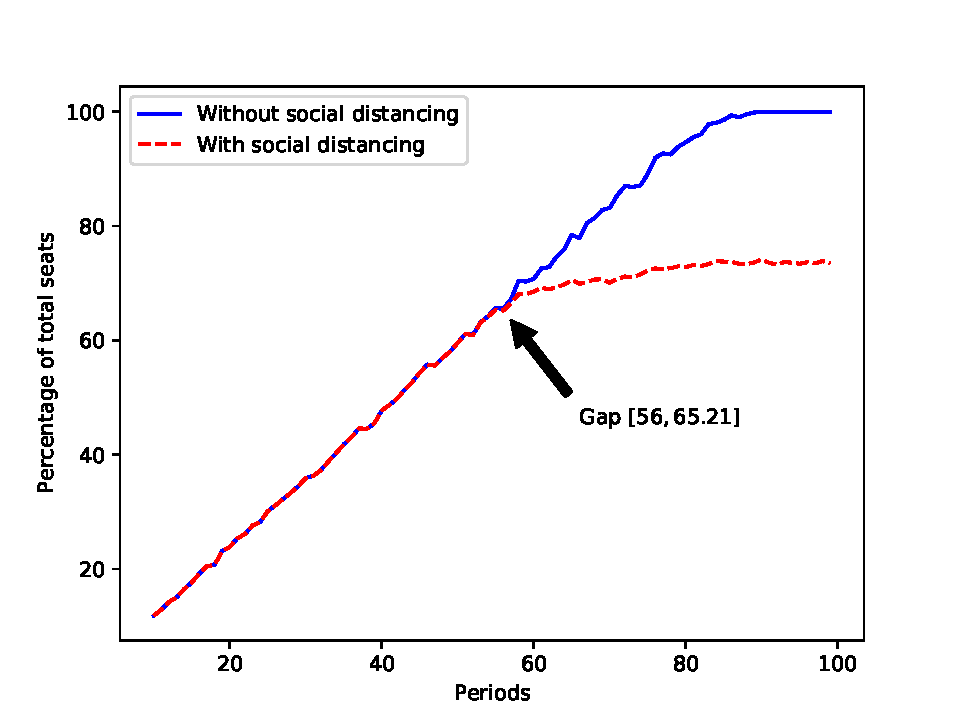
\includegraphics[width=0.48\textwidth]{./images/p1.pdf}}
            \subfigure[When $\gamma =1.9$]{
              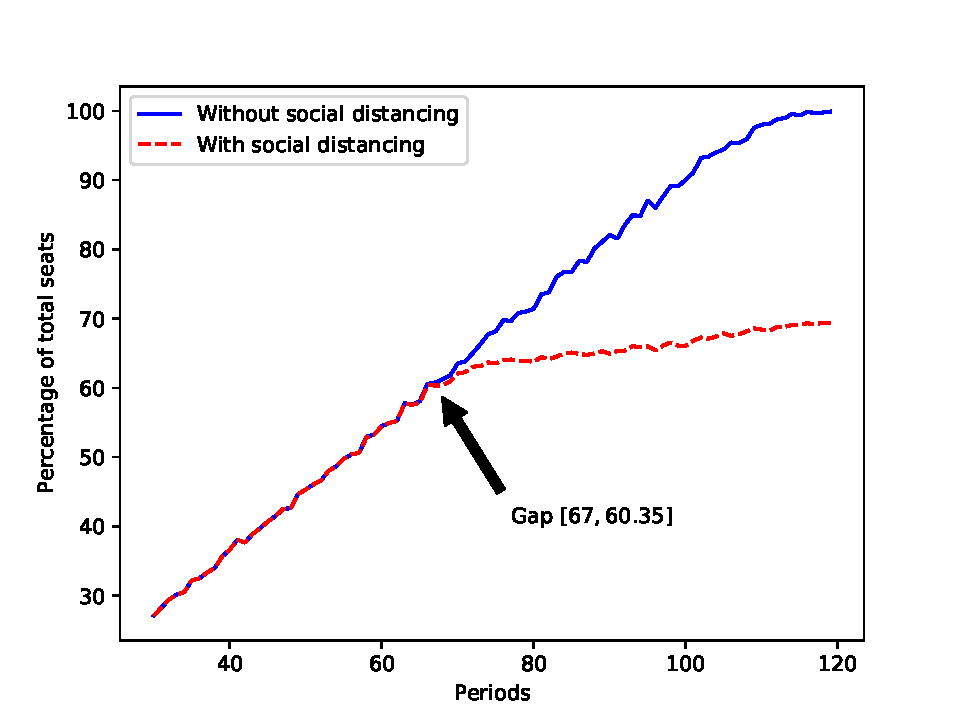
\includegraphics[width=0.48\textwidth]{./images/p2.pdf}}
          \end{figure}
        \scriptsize
        The gap point represents the first period where the number of people without social distancing is larger than that with social distancing and the gap percentage is the corresponding percentage of total seats.
    \end{frame}
      
    \begin{frame}{Estimation of Gap Point}
      \begin{figure}[ht]
        \centering
        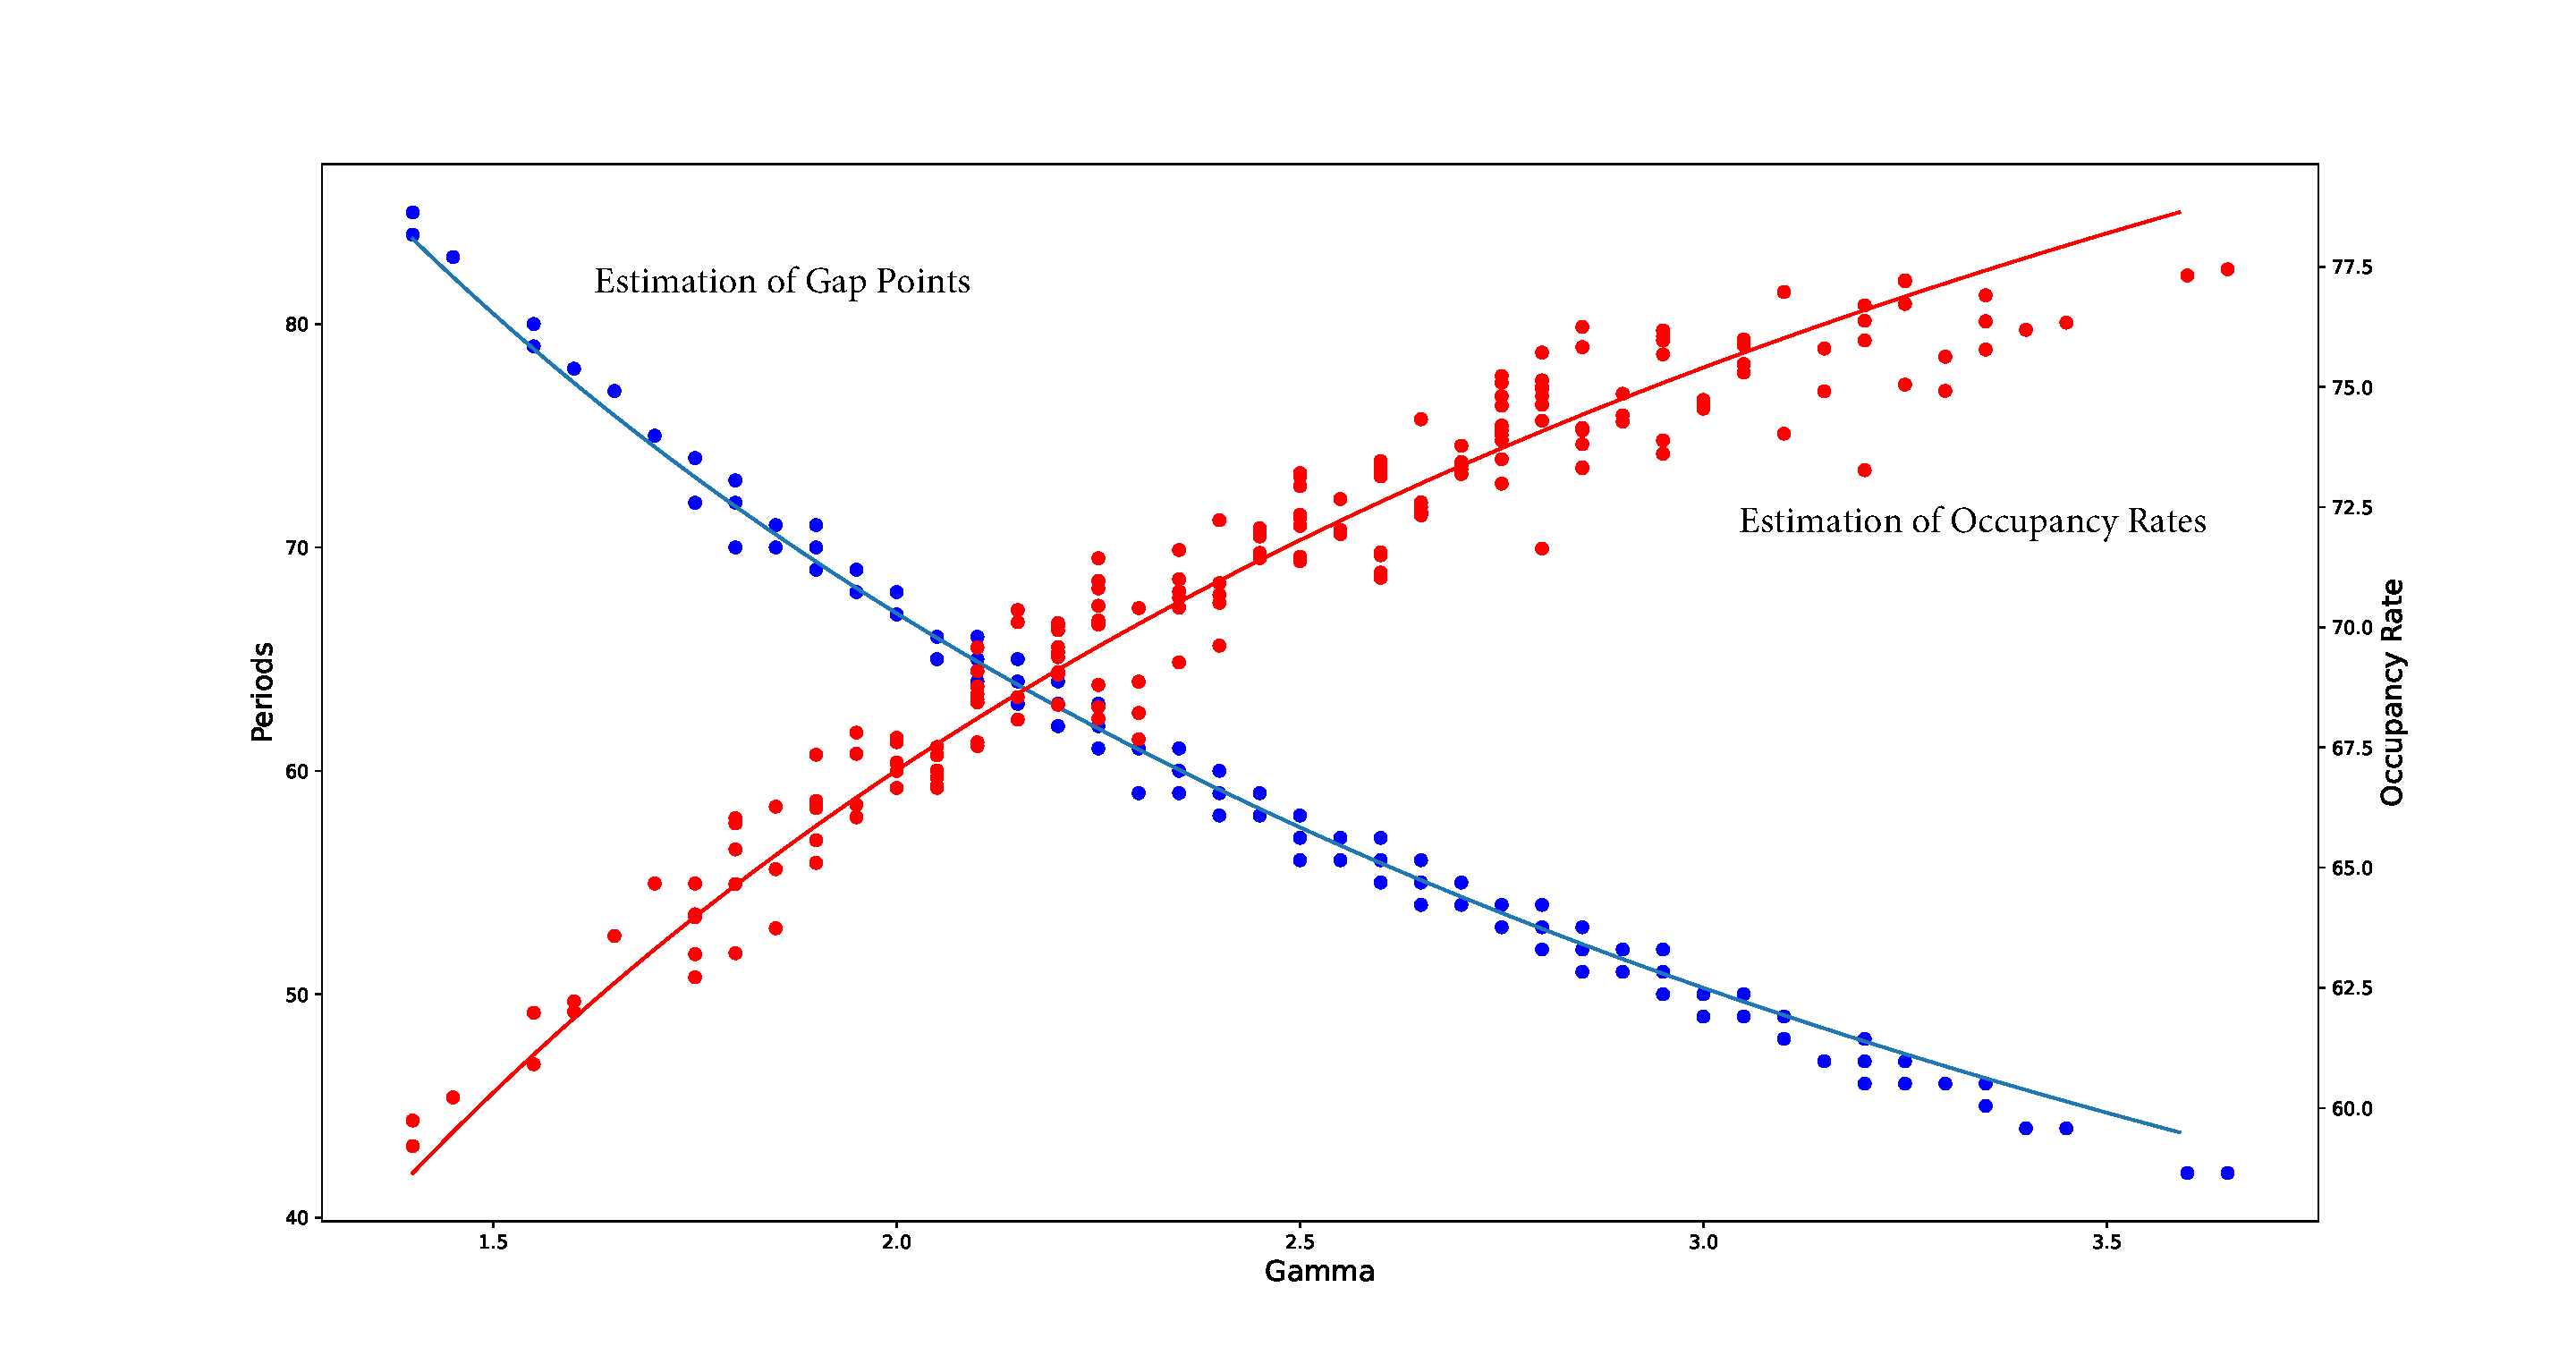
\includegraphics[width = 0.8\textwidth]{./images/gamma_estimation.pdf}
        \caption{Gap points with 200 probabilities}
    \end{figure}
    \scriptsize
    {\color{blue} Blue points}: period of the gap point.
    {\color{red} Red points}: occupancy rate of the gap point. 
    Gap points can be estimated.
    \end{frame}

    % We simulate 200 probabilities. For each probability, we run 100 instances to calculate the gap point and the corresponding occupancy rate. 
    
    % The point in the figure is the average of 100 instances. 
    % 


    \begin{frame}{Make A Later Allocation}
      This setting is particularly applicable to larger venues, such as stadiums, where an immediate decision is made when a group arrives, but the actual allocation of seats for that group is deferred to a later time.

      \vspace{0.5cm}

      The critical part is to make the decision, thus, we choose the following policies associated with relaxation forms.

      \vspace{0.5cm}

      Policies: 

      \begin{itemize}
        \item Dynamic programming based heuristic
        \item Bid-price control
      \end{itemize}
    \end{frame}

      \begin{frame}{Performances of Different Policies}
        \scriptsize
        \begin{table}[ht]
          \centering
          \begin{tabular}{|l|l|l|l|l|l|}
          \hline
           T & Probabilities &  DP1-L (\%) & Bid-L (\%) & DP1 (\%) & Bid (\%) \\
          \hline
          60  & [0.25, 0.25, 0.25, 0.25]  & 99.52 & 99.44 & 98.42 & 98.38 \\
          70  &   & 99.32 & 98.97 & 96.87 & 96.24 \\
          80  &   & 99.34 & 99.30 & 95.69 & 96.02 \\
          90  &   & 99.55 & 99.49 & 96.05 & 96.41  \\
          100 &   & 99.78 & 99.66 & 95.09 & 96.88 \\
          \hline
          60  & [0.25, 0.35, 0.05, 0.35]  & 99.50 & 99.37 & 98.26 & 98.25  \\
          70  &   & 99.40 & 98.97 & 96.62 & 96.06 \\
          80  &   & 99.46 & 99.24 & 96.01 & 95.89 \\
          90  &   & 99.59 & 99.35 & 96.77 & 96.62 \\
          100 &   & 99.77 & 99.61 & 97.04 & 97.14  \\
          \hline
          60  & [0.15, 0.25, 0.55, 0.05]  & 99.57 & 99.54 & 98.72 & 98.74 \\
          70  &   & 99.46 & 99.39  & 96.38 & 96.90 \\
          80  &   & 99.50 & 99.30  & 97.75 & 97.87 \\
          90  &   & 99.34 & 99.44  & 98.45 & 98.69 \\
          100 &   & 99.34 & 99.55  & 98.62 & 98.94 \\
          \hline
          \end{tabular}
        \end{table}

    \end{frame}

% !TEX root = sum1.tex
\section{Conclusion}
In conclusion, this paper addresses the problem of dynamic seat assignment with social distancing in the context of a pandemic. We propose a practical algorithm that balances seat utilization rates and the associated risk of infection to obtain a final seat planning that satisfies social distancing constraints when groups arrive. Our approach provides a comprehensive solution for optimizing seat assignments while ensuring the safety of customers. Our contributions include establishing a deterministic model to analyze the effects of social distancing when demand is known, using Benders decomposition methods to obtain the optimal solution for scenario-based stochastic programming, and developing a seat assignment policy for the dynamic situation. Our results demonstrate significant improvements over baseline strategies and provide guidance for developing attendance policies. Overall, our study highlights the importance of considering the operational significance behind social distancing and provides a new perspective for the government to adopt mechanisms for setting seat assignments to protect people in the post-pandemic era. Our study demonstrates the efficiency of obtaining the final seat planning using our proposed algorithm. The results indicate that our policy yields a seat planning that is very close to the optimal result. 

% Moreover, our analysis provides managerial guidance on how to set the occupancy rate and largest size of one group under the background of pandemic.


% \begin{table}[H]
%     \centering
%     \caption{xxxx}
%     \begin{tabular}{cccc}
%  \hline
%  a & aaaaaaaaa & aaaaaaaaaaaaaa & aaaaaaaaaaaaaaaaaaaa \\
%  \hline
%  a & \makebox[5ex][r]{123} & \makebox[6ex][r]{123456} & \makebox[6ex][r]{1}\\
%  a & \makebox[5ex][r]{12345} & \makebox[6ex][r]{123} & \makebox[6ex][r]{123} \\
%  a & \makebox[5ex][r]{1} & \makebox[6ex][r]{1234} & \makebox[6ex][r]{123456} \\
%  \hline
%  \end{tabular}
%  \end{table}

\bibliographystyle{plain}
\bibliography{refe}

% !TEX root = sum1.tex
\clearpage
\section*{Proof}

\begin{pf}[Proof of Proposition \ref{lem_pattern}]
First, we construct a feasible pattern with the size of $qM + \max\{r-\delta, 0\}$, then we prove this pattern is largest. We can utilize a greedy approach to construct a pattern, denoted as $\bm{h}_{g}$, by following the steps outlined below. This approach aims to generate a pattern that maximizes the number of people accommodated within the given constraints.

\begin{itemize}
 \item Begin by selecting the maximum group size, denoted as $n_M$, as many times as possible to fill up the available seats in the row.
 \item Allocate the remaining seats (if possible) in the row to the group with the corresponding size.
\end{itemize}

Let $L = n_M \cdot q + r$, where $q$ represents the number of times $n_M$ is selected (the quotient), and $r$ represents the remainder, indicating the number of remaining seats. It holds that $0 \leq r < n_M$. 

The number of people accommodated in the pattern $\bm{h}_{g}$ is given by $|\bm{h}_{g}| = q M + \max\{r-\delta, 0\}$. To establish the optimality of $|\bm{h}_{g}|$ as the largest number of people accommodated given the constraints of $L$, $\delta$, and $M$, we can employ a proof by contradiction.

% This expression takes into account the complete groups of size $M$ (represented by the product $q M$) and any remaining seats beyond the complete groups (represented by $\max{r-\delta, 0}$) that can be utilized to accommodate additional individuals, considering the social distancing requirement $\delta$.
% That is we need to prove $\max\{\sum_{i} (n_i - \delta)h_i| n_{i} h_{i} \leq L, h_{i} \in \mathbb{Z}\}$.

% With the capacity constraint, we have $L \geq \sum_{i} n_i h_i > \sum_{i} \delta h_i + q M + \max\{r-\delta, 0\}$. By substituting $L = n_M \cdot q + r$, we have $q(M + \delta) + r > \sum_{i} \delta h_i + q M + \max\{r-\delta, 0\}$.

Assuming the existence of a pattern $\bm{h}$ such that $|\bm{h}| > |\bm{h}_{g}|$, we can derive the following inequalities:

\begin{align*}
  & \sum_{i} (n_i - \delta) h_i > q M + \max\{r-\delta, 0\} \\
  \Rightarrow ~& L \geq \sum_{i} n_i h_i > \sum_{i} \delta h_i + q M + \max\{r-\delta, 0\} \\
  \Rightarrow ~& q(M + \delta) + r > \sum_{i} \delta h_i + q M + \max\{r-\delta, 0\} \\
  \Rightarrow ~& q \delta + r > \sum_{i} \delta h_i + \max\{r-\delta, 0\}
\end{align*}

Breaking down the above inequality into two cases:

\begin{enumerate}[(i)]
  \item When $r > \delta$, the inequality becomes $q+1 > \sum_{i} h_i$. It should be noted that $h_i$ represents the number of group type $i$ in the pattern. Since $\sum_{i} h_i \leq q$, the maximum number of people that can be accommodated is $q M < q M + r-\delta$.  
  \item When $r \leq \delta$, we have the inequality $q \delta + \delta \geq q \delta + r > \sum_{i} \delta h_i$. Similarly, we obtain $q+1 > \sum_{i} h_i$. Thus, the maximum number of people that can be accommodated is $q M$, which is not greater than $|\bm{h}_{g}|$.  
\end{enumerate}

Therefore, $\bm{h}$ cannot exist. The pattern, $\bm{h}_{g}$, is a largest pattern. The maximum number of people that can be accommodated in the largest pattern is $q M + \max\{r-\delta, 0\}$. 

% Correspondingly, the loss of the largest pattern $|\bm{h}_{g}|$ is $q \delta -\delta + \min\{r, \delta\}$.
\qed
\end{pf}

\begin{pf}[Proof of Proposition \ref{sol_relax_deter}]
  Treat the groups as the items, the rows as the knapsacks. There are $M$ types of items, the total number of which is $K = \sum_{i} d_i$, each item $k$ has a profit $p_k$ and weight $w_k$. 
  
  Then this Integer Programming is a special case of the Multiple Knapsack Problem (MKP). Consider the solution to the linear relaxation of \eqref{deter_upper}. Sort these items according to profit-to-weight ratios $\frac{p_1}{w_1} \geq \frac{p_2}{w_2} \geq \ldots \geq \frac{p_K}{w_K}$. 
  % $\delta$ is no less than 1, different types have
  Let the break item $b$ be given by $b=\min \{j: \sum_{k=1}^j w_k \geq L\}$, where $L = \sum_{j=1}^{N} L_j$ is the total size of all knapsacks. Then the Dantzig upper bound \cite{dantzig1957discrete} becomes $u_{\mathrm{MKP}}=\sum_{j=1}^{b-1} p_j+\left(L-\sum_{j=1}^{b-1} w_j\right) \frac{p_b}{w_b}$. The corresponding optimal solution is to accept the whole items from $1$ to $b-1$ and fractional $(L-\sum_{j=1}^{b-1} w_j)$ item $b$. Suppose the item $b$ belong to type $\tilde{i}$, then for $i < \tilde{i}$, $x_{ij}^{*} = 0$; for $i > \tilde{i}$, $x_{ij}^{*} = d_{i}$; for $i = \tilde{i}$, $\sum_{j} x_{ij}^{*} = (L - \sum_{i = \tilde{i}+1}^{M} {d_i n_i})/ n_{\tilde{i}}$. \qed
\end{pf}


% \begin{pf}[Proof of Proposition \ref{prop_onescenario}]
%   When $|\Omega| =1$ in SSP formulation, the stochastic programming will be 

%   \begin{equation}\label{one_form}
%     \begin{aligned}
%     \max \quad & \sum_{i=1}^{M}  \sum_{j= 1}^{N} (n_i-\delta) x_{ij} - \sum_{i=1}^{M} y_{i}^{+}  \\
%     \text {s.t.} \quad & \sum_{j= 1}^{N} x_{ij} - y_{i}^{+}+ y_{i+1}^{+} + y_{i}^{-} = d_{i}, \quad i = 1, \ldots, M-1, \\
%     & \sum_{j= 1}^{N} x_{ij} -y_{i}^{+} + y_{i}^{-} = d_{i}, \quad i = M, \\
%     & \sum_{i=1}^{M} n_{i} x_{ij} \leq L_j, j \in \mathcal{N}\\
%     & y_{i}^{+}, y_{i}^{-} \in \mathbb{Z}_{+}, \quad i \in \mathcal{M} \\
%     & x_{ij} \in \mathbb{Z}_{+}, \quad i \in \mathcal{M}, j \in \mathcal{N}.
%     \end{aligned}
% \end{equation}
  
%   To maximize the objective function, we can take $y_i^{+} = 0$. Notice that $y_{i}^{-} \geq 0$, thus the constraints $\sum_{j= 1}^{N} x_{ij} + y_{i}^{-} = d_{i}, i \in \mathcal{M}$ can be rewritten as $\sum_{j= 1}^{N} x_{ij} \leq d_{i}, i \in \mathcal{M}$. That is to say, problem \eqref{one_form} is equivalent to the deterministic model. \qed
% \end{pf}

\begin{pf}[Proof of Proposition \ref{prop_solution}]
  In any optimal solution where one of the corresponding patterns is not full or largest, we have the flexibility to allocate the remaining unoccupied seats. These seats can be assigned to either a new seat planning or added to an existing seat planning. Importantly, since a group can utilize the seat planning of a larger group, the allocation scheme based on the original optimal solution will not affect the optimality of the solution. 
  For each row, there are three situations to allocate the seats. First, when the rest seats can be allocated to the existing groups, then the corresponding pattern becomes a full pattern. Second, when all the existing groups are the largest groups and the rest seats cannot construct a new group, the pattern becomes the largest. Third, when all the existing groups are the largest groups and the rest seats can construct new groups, the rest seats can be used to construct the largest groups until there is no enough capacity, then the pattern becomes the largest. Finally, we can allocate the seats such that each row in the seat planning becomes either full or largest. \qed
  \end{pf}


\begin{pf}[Proof of Lemma \ref{feasible_region}]
% $W$ and $V$ are the totally unimodular matrix because 

Note that $\mathbf{f}^{\intercal} = [-\mathbf{1},~\mathbf{0}]$ and $V = [W,~I]$. Based on this, we can derive the following inequalities: $\bm{\alpha}^{\intercal}W \geq -\mathbf{1}$ and $\bm{\alpha}^{\intercal} I \geq \mathbf{0}$. These inequalities indicate that the feasible region is nonempty and bounded. Moreover, let $\alpha_0 = 0$. From this, we can deduce that $0 \leq \alpha_i \leq \alpha_{i-1} +1$ for $i \in \mathcal{M}$. Consequently, all extreme points within the feasible region are integral.
  \qed
\end{pf}

\begin{pf}[Proof of Proposition \ref{optimal_sol_sub_dual}]
  According to the complementary slackness property, we can obtain the following equations
  \begin{align*}
    & \alpha_{i} (d_{i0} - d_{i \omega} - y_{i \omega}^{+} + y_{i+1, \omega}^{+} + y_{i \omega}^{-}) = 0, i =1,\ldots, M-1 \\
    & \alpha_{i} (d_{i0} - d_{i \omega} - y_{i \omega}^{+}+ y_{i \omega}^{-}) = 0, i = M \\
    & y_{i \omega}^{+}(\alpha_{i} - \alpha_{i-1}-1) = 0, i =1,\ldots, M \\
    & y_{i \omega}^{-} \alpha_{i} = 0, i =1,\ldots, M.
  \end{align*}
  
  When $y_{i \omega}^{-} >0$, we have $\alpha_{i} =0$; when $y_{i \omega}^{+} >0$, we have $\alpha_{i} = \alpha_{i-1} +1$.
  Let $\Delta d = d_{\omega} - d_0$, then the elements of $\Delta d$ will be a negative integer, positive integer and zero.
  When $y_{i \omega}^{+} = y_{i \omega}^{-} = 0$, if $i = M$, $\Delta d_{M} =0$, the value of objective function associated with $\alpha_{M}$ is always $0$, thus we have $0 \leq \alpha_{M} \leq \alpha_{M-1}+1$; if $i < M$, we have $y_{i+1, \omega}^{+} = \Delta d_{i} \geq 0$. If $y_{i+1, \omega}^{+} > 0$, the objective function associated with $\alpha_i$ is $\alpha_{i} \Delta d_{i} = \alpha_{i} y_{i+1, \omega}^{+}$, thus to minimize the objective value, we have $\alpha_i =0$; if $y_{i+1, \omega}^{+} = 0$, we have $0 \leq \alpha_{i} \leq \alpha_{i-1} +1$.
  \qed
  \end{pf}

  \begin{pf}[Proof of Proposition \ref{one_ep_feasible}]
    Suppose we have one extreme point $\bm{\alpha}_{\omega}^{0}$ for each scenario. Then we have the following problem.
    \begin{equation}\label{lemma_eq}
      \begin{aligned}
        \max \quad & \mathbf{c}^{\intercal} \mathbf{x} + \sum_{\omega \in \Omega} p_{\omega} z_{\omega} \\
        \text {s.t.} \quad & \mathbf{n} \mathbf{x} \leq \mathbf{L} \\
        & (\bm{\alpha}_{\omega}^{0})^{\intercal}\mathbf{d}_{\omega} \geq (\bm{\alpha}_{\omega}^{0})^{\intercal} \mathbf{x} \mathbf{1} + z_{\omega}, \forall \omega \\
         & \mathbf{x} \in \mathbb{Z}^{+}_{0}
      \end{aligned}
    \end{equation}
    Problem \eqref{lemma_eq} reaches its maximum when $(\bm{\alpha}_{\omega}^{0})^{\intercal}\mathbf{d}_{\omega} = (\bm{\alpha}_{\omega}^{0})^{\intercal} \mathbf{x} \mathbf{1} + z_{\omega}, \forall \omega$. Substitute $z_{\omega}$ with these equations, we have 
    \begin{equation}\label{lemma_eq2}
      \begin{aligned}
        \max \quad & \mathbf{c}^{\intercal} \mathbf{x} - \sum_{\omega}p_{\omega}(\bm{\alpha}_{\omega}^{0})^{\intercal} \mathbf{x} \mathbf{1} + \sum_{\omega} p_{\omega} (\bm{\alpha}_{\omega}^{0})^{\intercal} \mathbf{d}_{\omega} \\
        \text {s.t.} \quad & \mathbf{n} \mathbf{x} \leq \mathbf{L} \\
        & \mathbf{x} \in \mathbb{Z}^{+}_{0}
      \end{aligned}
    \end{equation}
    Notice that $\mathbf{x}$ is bounded by $\mathbf{L}$, then the problem \eqref{lemma_eq} is bounded. Adding more constraints will not make the optimal value larger. Thus, RBMP is bounded. 
    \qed
  \end{pf}


% \begin{corollary}\label{coro_1}
%   Suppose there are two largest patterns, denoted as $h_1$ and $h_2$, with lengths $L_1 = n \cdot n_M$ and $L_2$ respectively (where $n$ is an integer), then $h_1 + h_2$ is largest with the length $L_1 + L_2$.
% \end{corollary}

% \begin{pf}[Proof of Proposition \ref{prop_construction}]
% To prove this proposition, we first prove the following lemma.

% \begin{lem}\label{generation}
%   For a feasible pattern $\bm{h}$ with $n$ groups and the length $L$, where $\sum_{i} n_{i} h_{i} \leq L \leq n \cdot n_{M}$, it is always possible to find a pattern $\bm{h}^{\prime}$ with $n$ groups which is the optimal solution to problem \eqref{gene_largest}. Additionally, $\bm{h}^{\prime}$ satisfies $|\bm{h}^{\prime}| = L - n$.
% \end{lem}
  
% \begin{pf}[Proof of Lemma \ref{generation}]
% We can demonstrate that the maximum value of $|\bm{h}^{\prime}|$ is $L - n$. For a feasible pattern $\bm{h}^{\prime}$ with $n$ groups, we have $\sum_{i}{h_i} = n$ and $\sum_{i}{n_i h_i} \leq L$. Therefore, we can deduce that $\sum_{i} {i h_i} \leq L - n$. To achieve equality, we need to transform the original pattern into a full pattern. Suppose the original pattern is not a full pattern. Let $\beta = L - \sum_{i} n_{i} h_{i}$, and identify the smallest group type in pattern $\bm{h}$ as $k$. We modify the original group of seats planned for $i$ people and allocate the unused seat(s) with the original group to accommodate $j$ people, where $j = \min\{M, \beta + i\}$. Let $\bm{h}^{1}$ represent the pattern after this allocation. As a result, we have $h^{1}_{i} = h_{i} -1$ and $h^{1}_{j} = h_{j} +1$. Thus, $\bm{h}^{1}$ will still satisfy the given constraints. This allocation process continues until $\beta$ reaches $0$. Eventually, we obtain a full pattern $\bm{h}^{\prime}$ that maximizes $|\bm{h}^{\prime}|$ while satisfying the constraints.
% \end{pf}

% Suppose there is a feasible pattern $\bm{h}$ with $n$ groups and the length $L_{j}$ for row $j$. When $L_{j} \leq n \cdot n_M$, Algorithm \ref{construction} can generate the optimal solution to problem \eqref{gene_largest} from Lemma \ref{generation}.

% When $L_{j} > n \cdot n_M$, Algorithm \ref{construction} can generate the pattern $\bm{h}^{\prime}$ which can be divided as $\bm{h}^{\prime} = \bm{h}^{\prime}_1 + \bm{h}^{\prime}_2$. The first part, $\bm{h}^{\prime}_1$, is associated with $L^1_{j} = n \cdot n_M$, the second part is associated with $L^2_{j} = L - n \cdot n_M$. According to Lemma \ref{generation}, $\bm{h}^{'}_1$ satisfies the constraints of problem \eqref{gene_largest}. Thus, $\bm{h}^{\prime}$ also satisfies these constraints. And $\bm{h}^{\prime}_2$ is a largest pattern according to Proposition \ref{lem_pattern}. Therefore, $\bm{h}^{\prime}$ is also a largest pattern.
% \end{pf}

\begin{pf}[Proof of Proposition \ref{prop_construction}]
First of all, we demonstrate the feasibility of problem \eqref{improve_seat}. Given the feasible seat planning $\bm{H}$ and $\tilde{d}_{i} = \sum_{j=1}^{N} H_{ji}$, let $\hat{x}_{ij} = H_{ji}, i \in \mathcal{M}, j \in \mathcal{N}$, then $\{\hat{x}_{ij}\}$ satisfies the first set of constraints. Because $\bm{H}$ is feasible, $\{\hat{x}_{ij}\}$ satisfies the second set of constraints and integer constraints. Thus, problem \eqref{improve_seat} always has a feasible solution. 

Suppose there exists at least one pattern $\bm{h}$ is neither full nor largest in the optimal seat planning obtained from problem \eqref{improve_seat}. Let $\beta = L - \sum_{i} n_{i} h_{i}$, and denote the smallest group type in pattern $\bm{h}$ by $k$. If $\beta \geq n_1$, we can assign at least $n_1$ seats to a new group to increase the objective value. Thus, we consider the situation when $\beta < n_1$. If $k =M$, then this pattern is largest. When $k< M$, let $h^{1}_{k} = h_{k} -1$ and $h^{1}_{j} = h_{j} +1$, where $j = \min\{M, \beta + i\}$. In this way, the constraints will still be satisfied but the objective value will increase when the pattern $\bm{h}$ changes. Therefore, by contradiction, problem \eqref{improve_seat} always generate a seat planning composed of full or largest patterns.

\end{pf}


\begin{pf}[Proof of Lemma \ref{bid-price}]
According to the Proposition \ref{sol_relax_deter}, the aggregate optimal solution to relaxation of problem \eqref{deter_upper} takes the form $x e_{h} + \sum_{i=h+1} ^{M} d_{i} e_{i}$, then according to the complementary slackness property, we know that $z_1, \ldots, z_h = 0$. This implies that $\beta_j \geq \frac{n_i - \delta}{n_i}$ for $i = 1,\ldots, h$. Since $\frac{n_i - \delta}{n_i}$ increases with $i$, we have $\beta_j \geq \frac{n_h - \delta}{n_h}$. Consequently, we obtain $z_{i} \geq n_i - \delta - n_i \frac{n_h - \delta}{n_h} = \frac{\delta(n_i-n_h)}{n_h}$ for $i = h+1, \ldots, M$.
  
Given that $\mathbf{d}$ and $\mathbf{L}$ are both no less than zero, the minimum value will be attained when $\beta_j = \frac{n_h - \delta}{n_h}$ for all $j$, and $z_i = \frac{\delta(n_i-n_h)}{n_h}$ for $i = h+1, \ldots, M$.  \qed
\end{pf}

% Problem \ref{bid-price_dual} can also be obtained by the following approximation:

% $V_{t}(\mathbf{L}) - V_{t+1}(\mathbf{L}) = \mathbb{E}_{i \sim p}\left[\max_{\substack{j \in \mathcal{N}: \\ L_j \geqslant {n}_{i}}}\left\{V_{t+1}\left(\mathbf{L}- n_{i}\mathbf{e}_j^{\intercal} \right)- V_{t+1}(\mathbf{L}) + i, 0 \right\}\right]$

% Approximation: $V_{t}(\mathbf{L}) = \theta^{t} + \sum_{j=1}^{N} L_j \beta_j$, substitute it to the above DP, we have 

% $V_{t}(\mathbf{L}) - V_{t+1}(\mathbf{L}) = \mathbb{E}_{i \sim p}\left[\max_{\substack{j \in \mathcal{N}: \\ L_j \geqslant {n}_{i}}}\left\{-n_i \beta_j + i, 0 \right\}\right] = \sum_i p_i \max_{j} \{-n_i \beta_j + i, 0\}$.

% Let $z_i = \max_{j} \{-n_i \beta_j + i, 0\}$, the constraints of dual form can be developed.

% The objective funtion: $V_{1} = \sum_{t=1}^{T} (V_{t} - V_{t+1}) = \sum_{i} d_{i} z_{i} + \sum_{j}^{N} L_{j} \beta_j$.

\newpage


% !TEX root = sum1.tex

\subsection{Obtain Minimum Number of Rows to Cover Demand}

To find the minimum number of rows to satisfy the demand, we can formulate this problem as a cutting stock problem form and use the column generation method to obtain an approximate solution.

Similar to the concept of pattern in the CSP, let the $k$-th placing pattern of a line of seats with length $S$ into some of the $m$ group types be denoted as a vector $(t^k_1,t^k_2,\ldots,t^k_m)$. Here, $t^k_i$ represents the number of times group type $i$ is placed in the $k$-th placing pattern. For a pattern $(t^k_1,t^k_2,\ldots,t^k_m)$ to be feasible, it must satisfy: $\sum_{i=1}^m t^k_i s_i \leq S$, where $s_i$ is the size of group type $i$. Denote by $K$ the current number of placing patterns.


This problem is to decide how to place a total number of group type $i$ at least $g_i$ times, from all the available placing patterns, so that the total number of rows of seats used is minimized.

Immediately we have the master problem:

\[\begin{split}\mbox{min}\quad & \sum_{k \in K}^K x_{k}\\
 \mbox{s.t.} \quad & \sum_{k \in K}^K t_i^k x_k \geq d_i  \quad  \mbox{ for } i=1,\ldots,m \\
  & x_k \geq 0, \mbox{integer}\quad \mbox{for}~ k \in K,\ldots,K.\\
\end{split}\]

If $K$ includes all possible patterns, we can obtain the optimal solution by solving the corresponding IP. But it is clear that the patterns will be numerous, considering all possible patterns will be time-consuming.

Thus, we need to consider the linear relaxation of the master problem, and the optimal dual variable vector $\lambda$. Using $\lambda$ as the value assigned to each group type $i$, the next problem is to find a feasible pattern $(y_1,y_2,\ldots,y_m)$ that maximizes the product of $\lambda$ and $y$.


Then the corresponding sub-problem is:
\[\begin{split}\mbox{max}\quad & \sum_{i=1}^m \lambda_i y_{i}\\
        \mbox{s.t.} \quad & \sum_{i=1}^m w_i y_i \leq S  \\
        & y_i \geq 0, \mbox{integer}\quad \mbox{for}~ i=1,\ldots,m.\\
\end{split}\]

This is a knapsack problem, its solution will be used as an additional pattern in the master problem.
We should continue to add new pattern until all reduced costs are nonnegative. Then we have an optimal solution to the original linear programming problem.

But note that column generation method cannot gaurantee an optimal solution. If we want to reach the optimal solution, we should tackle with the integer formulation.

\begin{equation}
\begin{aligned}
\min \sum_{k \in K}^{K} y_{k} & \\
\sum_{k=1}^{K} x_{i k} & \geq d_{i} \quad i=1, \ldots, n \\
\sum_{i=1}^{n} a_{i} x_{i k} & \leq S y_{k} \quad k=1, \ldots, K \\
y_{k} & \in\{0,1\} \quad k=1, \ldots, K \\
x_{i k} & \geq 0 \text { and integer } i=1, \ldots, n ; k=1, \ldots, K
\end{aligned}
\end{equation}

$y_k =1$ if line $k$ is used and 0 otherwise, $x_{ik}$ is the number of times group $i$ is placed in row $k$, and $K$ is the upper bound on the number of the rows needed.


\end{document}
